\chapter{Carbon-Neutral Community-Based Ride-sharing Framework}
\label{chapter3}

The European Green Deal has set the vision for a climate neutral continent by 2050 \cite{greendeal}.  For transportation systems to meet the aforementioned goal, a sustained transition to mass AEV and a fully RES-based energy market to power them is critical \cite{evplanning}. There is an onus on all citizens to play a role in this green transition; for example,  SECs are emerging to enable distributed energy generation and storage at a local level, representing a step further to the realisation of the term `Energy Citizen' \cite{energydatamanagement}.

Ride-sharing has presented new opportunities for the SEC sector to be productive with energy usage \cite{optimiserideshare}. Dynamic ride-sharing systems aim to match riders and drivers with similar itineraries and time schedules on short notice \cite{soa_rideshare}.
These systems can reduce the number of cars used for personal travel (improving the utilisation of available seat capacity) as well as the total distance for such travels, thus reducing the environmental impact.

The research presented in this chapter includes the design, implementation, and evaluation of a ride-sharing model operating in a smart city containing a number of SECs.

This aligns with the ambition of the EU Green Deal goals, and such a ride-sharing model envisions an alternative carbon-neutral,  community-based,  reactive transportation approach for managing city commutes using autonomous electric vehicles (AEVs).   
It targets  individual citizens (rather than on haulage/commercial transportation) that collectively aim to minimise their impact on the environment through the use of ride-sharing commutes while relying on a fleet of AEVs operating solely on RES. 

Specifically, the chapter includes the following contributions: 
\begin{enumerate}
    \item The formulation of a ride-sharing simulation model with the aforementioned conditions, presented as a variant of the classical Dynamic Vehicle Routing Problem with Time Windows \cite{vrp_survey}.  
    A number of SECs dispersed throughout the city provide the dynamic resources; each of them owns a number of autonomous AEVs and uses its own RES generation function to dynamically charge (and release) them over time. The ride-sharing service serves the dynamic requests provided via TPs, which are released over time. Each TP has its own location and pick-up/drop-off times. The formulation of the ride-sharing model integrates energy generation, allocation, and reactive re-routing constraints, with the objective function of maximising the overall number of TPs being served.  
    \item The design and implementation of the aforementioned ride-sharing model, with an algorithm following a reactive-based simulation approach on top of a greedy-based decision-making process. The algorithm favours scalability over optimality, with the aim for it to be applicable in real-world transportation of large cities. 
    \item The evaluation of the solution approach using a parameterised instance generator. It allows for the fine-grained customisation of (1) a Vehicle Routing Problem-based benchmark and (2) a public transportation-based dataset. Both (1) and (2) are adapted to  the specific requirements and format of the ride-sharing problem, testing the performance and scalability of the algorithm over a number of configurations. 
\end{enumerate}
In summary, this chapter introduces a complete framework for modelling, solving, and analysing a dynamic ride-sharing system powered by decentralised RES. It lays the groundwork for further enhancements in large-scale transportation networks, aiming for both environmental sustainability and operational efficiency.

\section{Mathematical Formulation}
\label{sec:proposed_system}

This section formalises the problem for a carbon-neutral, community-based reactive ride-sharing service as a variant of the classical Dynamic VRPTW. It integrates energy generation, allocation and reactive re-routing constraints as both the TPs and the number of available vehicles evolve during a simulated time horizon.  The ride-sharing service aims to maximise the number of TPs being served.  It is also intended to be highly scalable to facilitate transportation in large cities. 

The ride-sharing service contains the following features:
\begin{itemize}
\item The grid dimensions of the city $c_r$,  $c_c$ and the time horizon for the simulation $th$.  W.l.o.g.,  Manhattan distances among the locations of the city are assumed. 
\[
( c_r, c_c,  tih ) 
\]
\item A set S of SECs, each of them with an id $s_{id}$, a location in the city $s_x$,  $s_y$, a lexicographic-ordered list of the vehicles belonging to it $s_E$, the amount of vehicles ready at the start of the simulation (i.e., at time unit 0) $s_R$ and an energy function $fs_{id}:  \mathbb{N} x \mathbb{N}$ with the energy produced per time unit of the simulation, which will be used to release(in order) each new vehicle from $s_E$ as soon as enough energy to fill its battery capacity is generated. 
\[
( s_{id}, s_x, s_y, s_E,  s_R, fs_{id} ) \forall s\in S 
\]
\item A set E of AEVs, each of them with its own id $e_{id}$, the id of the SEC it belongs to $s_{id}$,  its release time during the simulation $e_{rt}$ (either 0 or when enough energy is generated) and its battery and passenger capacities ($e_{bc}$ and $e_{pc}$).  A mapping from E to S is assumed, such that each $e_{id}$ belongs to one $s_{id}$.
\[
( s_{id},  e_{id},  e_{rt},  e_{bc}, e_{pc} ) \forall e\in Es 
\]
\item A set T of TPs, each of them with its id $t_{id}$, its release time during the simulation $t_{rt}$ and its pick-up (resp. drop-off) locations $ t_{px}$, $ t_{py}$ (resp.  $ t_{dx}$, $ t_{dy}$) and time-windows $ t_{ep}$, $ t_{lp}$ (resp. $ t_{ed}$, $ t_{ld}$).  
\[
( t_{id},  t_{rt},  t_{px}, t_{py},  t_{ep}, t_{lp},  t_{dx}, t_{dy},  t_{ed}, t_{ld} ) \forall t\in T
\]
\end{itemize}

\subsection{Decision Variables}
\begin{itemize}
    \item $Alloc(t_{id}) \in E \cup \{-1\}$: Vehicle assigned to TP $t$, $-1$ if unassigned.
    \item $Sched(e_{id})$: Chronological sequence of movements for each AEV $e$.
\end{itemize}

\subsection{Objective Function}
\begin{equation}
\max \sum_{t \in T} \delta_t
\end{equation}

Where:
\[
\delta_t =
\begin{cases}
1, & \text{if } t_{id} \text{ is served within time windows} \\
0, & \text{otherwise}
\end{cases}
\]

\subsection{Constraints}
Following are the constraints: 
\begin{enumerate}
    \item \textbf{Vehicle Availability:} AEVs are released based on energy generation:    
    \[
    \sum_{t' = 0}^{e_{rt}} fs_{id}(t') \geq e_{bc}, \quad \forall e \in E
    \]
    \item \textbf{Battery Dynamics:} For each movement $m_i \in Sched(e_{id})$:
    \[
    EE_i = ES_i - d(AX_i, AY_i, BX_i, BY_i)
    \]
    Where $d(\cdot)$ is the Manhattan distance.
    \item \textbf{Passenger Constraints:} Pick-ups and drop-offs update $PS_i$ accordingly.
    \[
    0 \leq PE_i \leq e_{pc}
    \]
    \item \textbf{Time Window Satisfaction:} For TP $t$ to be served:
    \[
    t_{ep} \leq TA_{pickup} \leq t_{lp}
    \]
    \[
    t_{ed} \leq TA_{dropoff} \leq t_{ld}
    \]
    \item \textbf{Allowed Movement Types:} \[
    Tl_i =
    \begin{cases}
    +t_{id}, & \text{pick-up for TP} \\
    -t_{id}, & \text{drop-off for TP} \\
    \text{idle}, & \text{vehicle idle period} \\
    \text{ret}, & \text{return to home SEC}
    \end{cases}
    \]
\end{enumerate}

\subsection{Output}
The ride-sharing service is intended to provide an output containing the following features:
\begin{itemize}
    \item A set Alloc, representing an allocation mapping from T to E. 
    \[
    \forall t\in T
    \text{ }Alloc[t_{id}] = 
    \begin{cases}
        e_{id},  \text{if }  t_{id} \text{ is allocated to } e_{id}\\
        -1,  \text{otherwise}
    \end{cases}
    \]
    \item A set Sched, representing a scheduling mapping from E to its sequence of movements (in chronological order) over the entire time horizon. 
    \[
    \forall e\in E
    \text{ }Sched[e_{id}] = ( m_0,  m_1,  \ldots,  m_{n-1} ) 
    \]
    Each movement $m_i$ of a vehicle is represented as
    \begin{align*}
    m_i \equiv \{ ( TA_i, TB,_i AX_i, AY_i, BX_i, BY_i, PS_i, \\
        PE_i, ES_i, EE_i, TL_i, LW_i, TD_i ) \} \\  
    \end{align*}	
    with: 
\begin{itemize}
    \item $TA_i$ (resp. $TB_i$) represent the start time (resp.  end time) of $m_i$. 
    \item $AX_i$ and $AY_i$ (resp.   $BX_i$ and $BY_i$) represent the coordinates of the vehicle at the start (resp. end) of $m_i$.
    \item $PS_i$ (resp. $PE_i$) represents the number of passengers in the vehicle at the start time (resp. end time) of $m_i$. 
    \item $ES_i$ (resp. $EE_i$) represents the battery left in the vehicle at the start time (resp. end time) of $m_i$. 
    \item $Tl_i$ represents a label to identify the purpose of the trip. 
    \begin{itemize}
    \item A movement for picking-up (resp. dropping off) the passenger of $t_{id}$ is marked as $+t_{id}$ (resp.  $-t_{id}$).
    \item An idle movement (resting at a given location) is marked as $idle$. 
    \item A last movement, returning to its home SEC is marked as $ret$.  
    \end{itemize}
    \item $LW_i$ represents the leeway of the movement, i.e., the maximum delay that could be applied to the movement while still accomplishing the action is intended to. 
    \item $TD_i$ represents the movement duration. 
\end{itemize}
\end{itemize}
The proposed carbon-neutral, community-based ride-sharing problem extends the classical DVRPTW, which is well-established as NP-Hard. The additional integration of decentralised SECs, RES generation constraints, battery dynamics, and reactive vehicle scheduling further increases the problem's computational complexity.

Consequently, the category of the problem is NP-Hard. While the current formulation is an optimisation problem aimed at maximising the number of served TPs, a corresponding decision version—determining whether at least $k$ TPs can be served within all constraints—would be NP-Complete, assuming polynomial-time verifiability of candidate solutions \cite{hasan2020commute}.



% \textbf{5. Movement Continuity:}

% \[
% (BX_i, BY_i) = (AX_{i+1}, AY_{i+1})
% \]
% \[
% TB_i = TA_{i+1}
% \]

% \textbf{6. Charging Dynamics at SECs:}

% Battery is replenished at SECs based on available energy $fs_{id}(t)$.


% \subsection{Problem Summary}

% The problem jointly optimises vehicle scheduling, energy allocation, and trip assignments to maximise served TPs, respecting:
% \begin{itemize}
%     \item Energy generation and consumption constraints.
%     \item Passenger capacity and ride-sharing conditions.
%     \item Pick-up and drop-off time windows.
%     \item Geographic vehicle distribution among SECs.
% \end{itemize}

% The resulting system enables scalable, carbon-neutral, community-based ride-sharing under decentralised and dynamic urban conditions.


\subsection{Instance Example}
\label{instance_example}

To highlight the approach taken, an example of a problem instance is presented here. It represents a city of dimensions 3 x 4 (w.l.o.g, 3km x 4km) and a simulated time horizon of 10 units (w.l.o.g., 10 minutes).  
\[
( c_r = 3, c_c = 4,  th = 10 ) 
\]
The city contains just 1 SEC,  with id $SEC_1$ and placed at location (1,2),  with a list of 2 vehicles $S_E \equiv [ AEV_1, AEV_2]$, one vehicle ready to go at the start of the simulation,  and a constant energy generation function of 2kWh per time unit $fSEC_1 = 2$.
\[
 S \equiv \{ ( SEC_1, 1, 2, [AEV_1, AEV_2], 1,  fSEC_1) \}
\]
A constant speed is assumed, making each vehicle to traverse 1 block of the city every time unit, while consuming 1 unit of its battery capacity (w.l.o.g., 60km/h constant speed and 60kWh constant consumption).  
Both AEVs have a battery capacity of 10kWh and room for 5 passengers.  Whereas $AEV_1$ is released at the start of the simulation (time unit 0),  $AEV_2$ is released when its battery capacity is generated by $SEC_1$ (i.e., given the constant energy generation of 2kWh per time unit,  the vehicle is generated at time unit 5).  If $SEC_1$ had had more vehicles in $S_E$, they would have been released (in order) at time units 10, 15, and so on.
\[
E \equiv \{ ( SEC_1,  AEV_1,  0,  10,  5 ),  ( SEC_1,  AEV_2,  5,  10,  5 ) \}
\]
The city receives 3 TPs,  with ids $TP_1$,  $TP_2$ and $TP_3$. 
$TP_1$ is announced at time unit 0,  to pick-up the passenger at location (2,3) between time units 0 and 4, and to drop-off at location (0,0) between time units 5 and 7. 
$TP_2$ is announced at time unit 2,  to pick-up the passenger at location (2,2) between time units 3 and 4, and to drop-off  at location (1,1) between time units 5 and 6. 
$TP_3$ is announced at time unit 6,  to pick-up the passenger at location (2,3) between time units 6 and 7, and to drop-off  at location (1,3) between time units 7 and 9. 
\begin{align*}
T \equiv \{ (TP_1,  ( 0, 2, 3, 0, 0, 0, 4, 5, 7 )), \\
			      (TP_2, ( 2, 2, 1, 1, 1, 3, 4, 5, 6 )), \\
			      (TP_3, ( 6, 2, 3, 1, 3, 6, 7, 7, 9 )) \}		      
\end{align*}
A feasible solution to this instance allocates $TP_1$ and $TP_2$ to $AEV_1$, while $TP_3$ is not allocated.
\[
Alloc \equiv \{ (TP_1, AEV_1),  (TP_2, AEV_1),  (TP_3, -1) \}
\]

In the allocation above,  the vehicles have the following schedules: 
\begin{align*}
Sched \equiv \{ (AEV_1,  [ ( 0, 2, 1, 2, 2, 3, 0, 1, 10, 8, +TP_1, 2, 2 ), \\
									  ( 2, 4, 2, 3, 2, 1, 1, 2, 8, 6, +TP_2, 0, 2 ), \\
									  ( 4, 5, 2, 1, 1, 1, 2, 1, 6, 5, -TP_2, 1, 1 ), \\
									  ( 5, 7, 1, 1, 0, 0, 1, 0, 5, 3, -TP_1, 0, 2 ), \\									 
									  ( 7, 10, 0, 0, 1, 2, 0, 0, 3, 0, ret, 0, 3 )]),\\										 
							(AEV_2,  [ ( 5, 10, 1, 2, 1, 2, 0, 0, 10, 10, idle, 5, 0 )	] \} \\  
\end{align*}							       
	
Figure \ref{fig:sched_instance_example} displays the route of $AEV_1$ and $AEV_2$ in $Sched$. W.l.o.g.,  the coverage of the Manhattan distance between two points is assumed to be traversed always by covering first the distance of the x-axis followed up by the distance in the y-axis.  The release of an AEV is highlighted in blue, an idle movement in grey and an active movement  by its starting point (green) and destination one (red). 
\begin{figure}[b]
  \vspace{-0.2cm}
  \centering
   {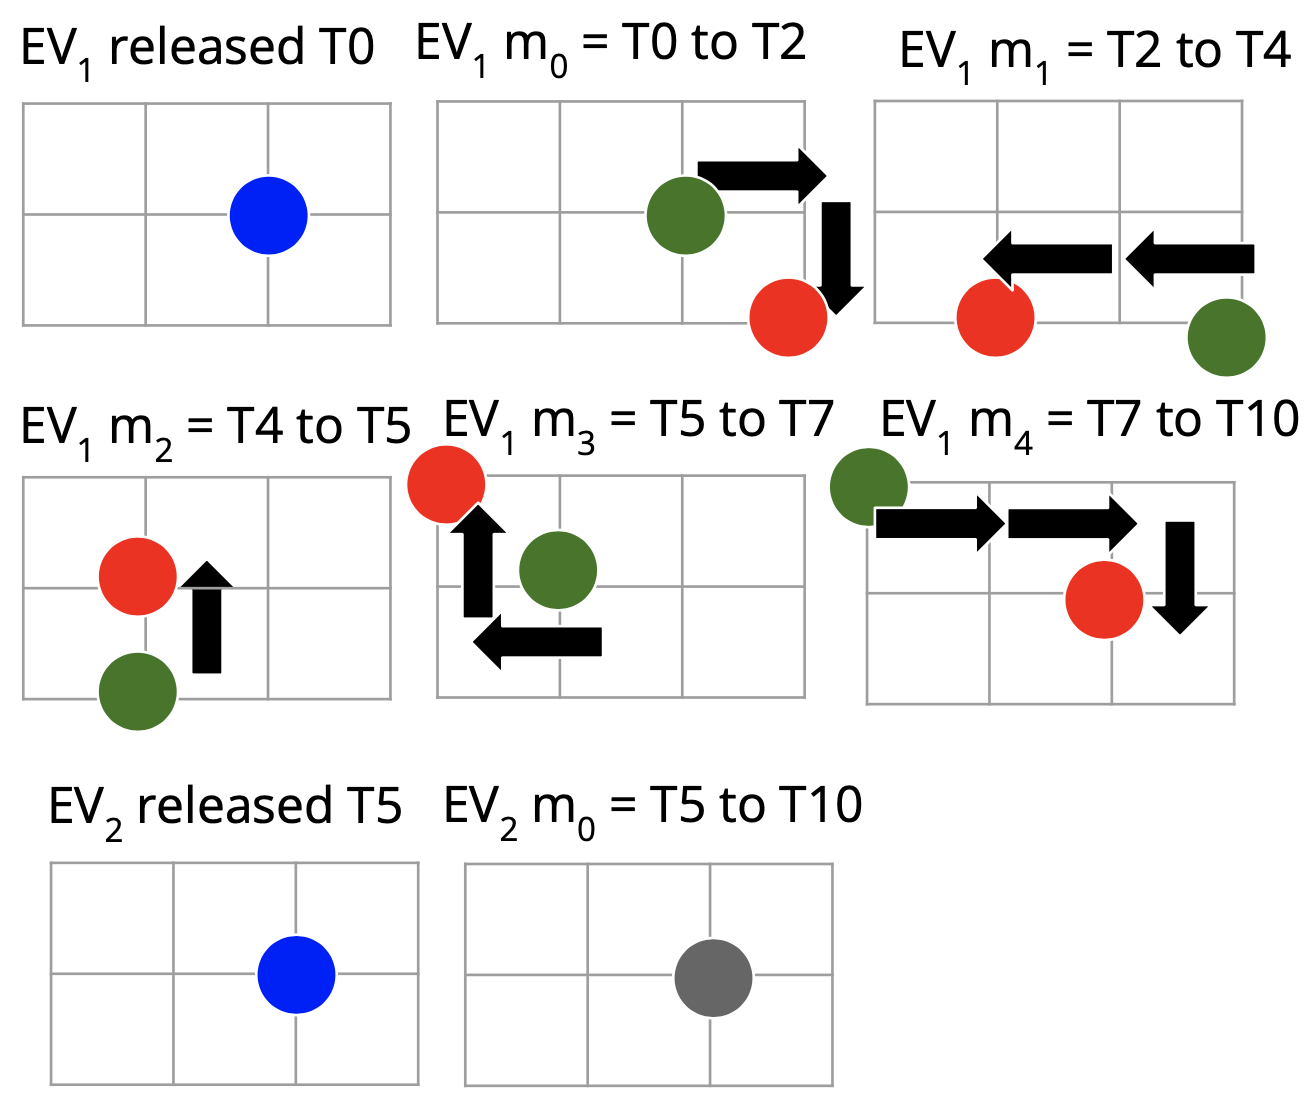
\epsfig{file = Crest/Images/sched.png, width = 0.5\textwidth}}
  \caption{$Sched$ Outputted as Solution}
  \label{fig:sched_instance_example}
    \vspace{-0.1cm}
\end{figure}	
	
The route of $AEV_1$ is composed of 5 movements:									 										 			
\begin{enumerate}
\item From time unit 0 to time unit 2, it leaves the $SEC_1$ to serve the pick-up of $TP_1$.  On doing so,  it goes from (1,2) to (2,3), increases its number of passengers from 0 to 1, and reduces its battery capacity from 10 to 8.  As the pick-up of $TP_1$ must be within time units 0 and 4 and $AEV_1$ arrives at time unit 2,  a leeway of 2 time units is associated to the movement, as it could have been re-scheduled by delaying it up to 2 time units in case the vehicle had needed any re-routing. 
\item From time unit 2 to time unit 4, the vehicle serves the pick-up of $TP_2$.  On doing so,  it goes from (2,3) to (2,1), increases its number of passengers from 1 to 2, and reduces its battery capacity from 8 to 6.  As the pick-up of $TP_2$ must be within time units 3 and 4 and $AEV_1$ arrives at time unit 4,  a leeway of 0 time units is associated to the movement, as it cannot be further delayed by any re-routing.
\item From time unit 4 to time unit 5, the vehicle serves the drop-off of $TP_2$.  On doing so,  it goes from (2,1) to (1,1), decreases its number of passengers from 2 to 1, and reduces its battery capacity from 6 to 5.  As the drop-off of $TP_2$ must be within time units 5 and 6 and $AEV_1$ arrives at time unit 5,  a leeway of 1 time unit is associated to the movement.
\item From time unit 5 to time unit 7, the vehicle serves the drop-off of $TP_1$.  On doing so,  it goes from (1,1) to (0,0), decreases its number of passengers from 1 to 0, and reduces its battery capacity from 5 to 3.  As the drop-off of $TP_1$ must be within time units 5 and 7 and $AEV_1$ arrives at time unit 7,  a leeway of 0 time units is associated to the movement.
\item From time unit 7 to time unit 10, the vehicle returns to $SEC_1$ before the end of the simulation.  On doing so,  it goes from (0,0) to (1,2), stays at 0 passengers, and reduces its battery capacity from 3 to 0.  As the end of the time horizon is at time unit 10, and the vehicle arrives to $SEC_1$ at time unit 10,  a leeway of 0 time units is associated to the movement.
\end{enumerate}

The route of $AEV_2$ is composed of just 1 movement, as the vehicle remains idle since it is released at time unit 5 until the end of the time horizon. 


\section{Solution Approach}
\label{sec:solution_approach:chap2}

This section presents an initial algorithm to solve the problem formalised in Section \ref{sec:proposed_system}.  Subsections \ref{detailed_explanation} and \ref{complexity_analysis} present the algorithm and analyse its complexity, respectively.

\subsection{Algorithm Overview}
\label{detailed_explanation}

Given a valid instance of a city with its SECs, vehicles, energy generation and TPs, the algorithm aims to maximise the number of TPs being served, outputting both the allocation of each trip to a vehicle and the routing of each vehicle over the entire simulated time horizon. To do so, the algorithm implements a reactive simulation approach on top of a greedy decision-making process for trip allocations.  Algorithm 1 presents the pseudocode of the solution approach, which is explained in detail next. 
\begin{algorithm}\captionsetup{labelfont={sc,bf}}
\caption{- Ride-Sharing}
\begin{small}
\begin{algorithmic}
\Function{$allocate$}{$e$, $t$, $Alloc[t]$, $Sched[e]$} 
\State $is\_allocated\gets false$
\State $m \equiv [ m_0, \ldots, m_{k-1} ] \gets copy(Sched[e])$
\For{$i \in 0, \ldots, k-1$}
	\If{$pick\_up(m, t, i)$}
		\State $m\gets [ m_0, \ldots,  m_i', m_{i+1}', \ldots,  m_{r-1}' ]$
		\For{$j \in i+1, \ldots, r-1'$}
			\If{$drop\_off(m, t, j)$}	
				\State $m\gets [ m_0,  \ldots, m_j'',  m_{j+1}'', \ldots,  m_{w-1}'' ]$	
				\If{$ret\_sec(m, w-1)$}
					\State $m\gets [ m_0,  \ldots, m_{w-1}'', m_w'' ]$
					\State $(Alloc[t], Sched[e]) \gets (e, m)$
					\State $is\_allocated \gets true$	
				\EndIf
				\State $Break$				
			\EndIf	
		\EndFor
		\State $Break$
	\EndIf
\EndFor
\Return $is\_allocated$
\EndFunction
\\\hrulefill
\end{algorithmic}
\begin{algorithmic}
\Function{$reactive\_simulation$}{$S$, $E$, $T$, $th$} 
\State $(Alloc, Sched)\gets init(S, E, T, th)$
\For{$t \in sorted(T)$}
	\For{$e \in E$}
		\If{$allocate(e, t, Alloc[t], Sched[e])$}
			\State $Break$
		\EndIf
	\EndFor	
\EndFor
\Return $(Alloc, Sched)$
\EndFunction
\end{algorithmic}
\end{small}
\end{algorithm}



\subsubsection{Reactive-Based Simulation}
\label{reactive_based_simulation}

First, the algorithm initialises $Alloc$, considering each trip as initially not allocated.  It also initialises $Sched$, considering the route of each vehicle as, initially, resting at its home SEC from its release time $e_{rt}$ to the end of the time horizon of the simulation $th$.  
Therefore,  even at the beginning of the simulation (time unit 0), all vehicles have an associated schedule (even if such schedule does not start until a release time unit $e_{rt}$ in the future). 
\[
\forall t\in T\text{ }Alloc[t_{id}] = (e_{id}, -1) 
\]
\begin{align*}
\forall e\in E \text{ } \exists s_{id} \in S \text{ with } s_x, s_y, s_E, e\in s_E \text{ s.t.  } Sched[e_{id}] =\\ 
[( e_{rt}, th, s_x, s_y, s_x, s_y, 0, 0, e_{bc}, e_{bc}, idle, th-e_{rt}, 0 )]
\end{align*}	
For example, given the instance of Section \ref{instance_example}, the initial value of $Alloc$ and $Sched$ is as follows: 
\[
Alloc \equiv \{ (TP_1, -1),  (TP_2, -1),  (TP_3, -1) \}
\]
\begin{align*}
Sched \equiv \{(AEV_1,  [ ( 0, 10, 1, 2, 1, 2, 0, 0, 10, 10, idle, 10, 0 )]\\										 
(AEV_2,  [ ( 5, 10, 1, 2, 1, 2, 0, 0, 10, 10, idle, 5, 0 )] \}\\ 
\end{align*}	

The algorithm then simulates a reactive-based ride-sharing service by simply sorting all TPs by their increasing release time (referred to as $sorted(T)$),  thus attempting to serve each TP as soon as it is released.  For each $t \in sorted(T)$, the algorithm iterates for each $e \in E$, attempting to allocate the trip to the vehicle by dynamically re-routing its schedule (i.e., by fitting both the pick-up and drop-off of $t$ as new movements into the existing schedule of the vehicle $Sched[e]$.  As soon as the algorithm successfully allocates $t$ to a vehicle $e$,  the search stops (i.e., the trip is not attempted to be allocated to any other vehicle). On the other hand, if no vehicle can allocate $t$, then the attempt to serve the TP is considered as not successful, and no further attempt for allocating it is made for the rest of the simulation. 

For example, given the instance of Section \ref{instance_example}, the trips $TP_1$, $TP_2$ and $TP_3$ are released in time units 0,  2 and 6, respectively.  Therefore: 
\begin{enumerate}
\item The algorithm simulates that $TP_1$  is attempted to be allocated first, at time unit 0.  On that moment, the schedule of $AEV_1$ and $AEV_2$ is the initial one described above.  If $AEV_1$ can be successfully re-routed to fit $TP_1$, then it is allocated to it. Otherwise $AEV_2$ is attempted.  If $TP_1$ can not be serviced by either $AEV_1$ or $AEV_2$, then $TP_1$ is not allocated.  In any case, these allocation attempts lead to a new updated state $Sched'$ and $Alloc'$.
\item The algorithm continues by attempting to allocate $TP_2$ over $AEV_1$ first and $AEV_2$ otherwise with their current updated schedules $Sched'$ at time unit 2,  further leading to a new updated state $Sched''$ and $Alloc''$.
\item Finally, the algorithm continues by attempting to allocate $TP_3$ over $AEV_1$ first and $AEV_2$ otherwise with their current updated schedules $Sched''$ at time unit 6, leading to the final state (the one reported as output) $Sched'''$ and $Alloc'''$.
\end{enumerate} 

\subsubsection{TP Allocation}
\label{fitting_into_sched}

The allocation of $t$ to $e$ (specifically, to its schedule $Sched[e]$) is defined to be successful if: 
\begin{enumerate}
\item The updated $Sched[e]'$ incorporates one new movement ensuring the pick-up (resp. drop-off) of $t$ within its defined time window $t_{ep}$ and $t_{lp}$ (resp.  $t_{ed}$ and $t_{ld}$). The functions $pick\_up$ (resp. $drop\_off$) ensure this (cf.  Algorithm 1). 
\item The updated $Sched[e]'$ contains a very last active movement, labelled as $ret$, ensuring the vehicle returning to its home SEC before the end of the time horizon $th$.  The functions $ret\_sec$ ensures this (cf.  Algorithm 1). 
\item The addition of these new pick-up, drop-off and ret movements to $Sched[e]'$ (to serve $t$) might delay the actual pick-up and drop-off times of any other previous trips $t_z$ the vehicle $e$ had previously committed to. For $t$ to be successfully allocated to $e$, such as these additional delays on serving $t_z$ must not break the pick-up and drop-off time windows of $t_z$.  In other words, once a vehicle $e$ commits to a trip $t_z$,  no further trip allocation $t$ can delay $e$ enough to make it not serving $t_z$ in time. The functions $pick\_up$ (resp. $drop\_off$) ensure this (cf.  Algorithm 1).  
\item The updated $Sched[e]'$ contains no movement where the number of passengers exceeds its capacity $e_{pc}$ or where the battery capacity $e_{bc}$ goes below 0. 
\end{enumerate} 

To fit $t$ into $Sched[e] = [ m_0, \ldots, m_{k-1} ]$ 
the algorithm iterates through its movements (which are in chronological order).  When considering a movement 
$m_a \equiv (TA_a, TB_a,  ... )$, the algorithm only considers its starting time unit $TA$ (i.e., the decision of whether to re-route or not $e$ to serve $t$ is considered just at $TA$, not at any other given time in the 
interval $(TA,\ldots,TB]$.  

First, the algorithm searches for a movement $m_i$ fitting the pick-up of $t$.  As soon as such movement $m_i$ is found, no further movement $m_j$ with $j > i$ of $e$ is considered for picking-up $t$, and the algorithm moves on into searching for a movement $m_j$ fitting the drop-off of $t$.  Again, as soon as such movement $m_j$ is found, no further movement $m_k$ with $k > j$ of $e$ is considered for dropping-off $t$.  

Needless to say,  both policies (1) considering just the starting time $TA$ of each movement and the policy (2) considering just one valid pair ($m_{i}$, $m_{j}$) of picking-up and dropping-off movements make the search incomplete. That is, the search is not considering other ($m_{i'}$, $m_{j'}$) valid combinations and any other valid re-routing times for such combinations other than $TA_{i'}$ and $TA_{j'}$. Any such alternatives might lead not only to the allocation of $t$, but to an overall higher number of trips allocated, which is the goal aimed at by the algorithm. However, these policies (1) and (2) are designed to favour scalability over optimality for the algorithm (more detail in Section \ref{complexity_analysis}). 
Moreover, although not leading to optimality, the above non-complete search still leads to a very competitive trip allocation rate when applied to real-world very large instances, as it is discussed in more detail in Section \ref{analysis_performance}.  

Given the instance of Section \ref{instance_example}, the following analyses the attempt to fit $TP_2$ into $AEV_1$ at time unit 2.  
\[
TP_2 \equiv ( 2, 2, 1, 1, 1, 3, 4, 5, 6 )
\]
As described previously,  at this stage in the simulation,  $TP_1$ had been successfully allocated to $AEV_1$, making its $Sched[AEV_1]$:
\begin{align*}
Sched[AEV_1] = [\\ 
m_0 \equiv ( 0, 2, 1, 2, 2, 3, 0, 1, 10, 8, +TP_1, 2, 2 ),\\
m_1 \equiv ( 2, 7, 2, 3, 0, 0, 1, 0, 8, 3, -TP_1, 0, 5 ),\\
m_2 \equiv ( 7, 10, 0, 0, 1, 2, 0, 0, 3, 0, ret, 0, 3 )] 									 
\end{align*}	 

The window of opportunity for allocating the pick-up of $TP_2$ is from $TP2_{rt} = 2$ to $TP2_{lp} = 4$. 

The algorithm first attempts to fit the pick-up on $m_0$, but fails, as the time of the movement $TA_0$ is 0, even before $TP_2$ is announced, and therefore outside of its window of opportunity.  

The algorithm then attempts $m_1$, and it succeeds. $m_1$ spans from time unit $TA_1 = 2$ to $TB_1 = 7$, going from (2,3) to (0,0) for dropping-off $TP_1$.  The total distance covered is 5. It must be at (0,0) at time unit 7 at the latest ($TP1_{ld} = 7$), so it cannot be further delayed.  Re-routing $m_1$ to serve pick-up of $TP_2$ involves (1) going from (2,3) to (2,1); (2) arrive there between time units 3 and 4; (3) going from (2,1) to (0,0); (4) still arrive there on time (i.e., time unit 7 + 0 leeway = 7). The total distance of re-route to pick-up $TP_2$ while still dropping-off $TP_1$ from there is 2 + 3 = 5; if leaving straight-away at time unit 2, it will reach (2,1) to pick-up $TP_2$ at time unit 4, still within the window of opportunity, and leading to a leeway of 0, as this new movement cannot be any further delayed. 

The new state of $Sched'[AEV_1]$ is: 
\begin{align*}
Sched'[AEV_1] = [\\
m_0' \equiv ( 0, 2, 1, 2, 2, 3, 0, 1, 10, 8, +TP_1, 2, 2 ),\\
m_1' \equiv ( 2, 4, 2, 3, 2, 1, 1, 2, 8, 6, +TP_2, 0, 2 ),\\
m_2' \equiv ( 4, 7, 2, 1, 0, 0, 2, 1, 6, 3, -TP_1, 0, 3 )\\ 
m_3' \equiv ( 7, 10, 0, 0, 1, 2, 0, 0, 3, 0, ret, 0, 3 )]										 
\end{align*}	

The window of opportunity for allocating drop-off of $TP_2$ is from the next time unit to its pick-up (5) to $TP2_{ld} = 6$. 

The algorithm first attempts $m_2'$ (as it does not start attempting the drop-off allocation any earlier than the pick-up movement), and it succeeds.  $m_2'$ spans from time unit $TA_2' = 5$ to $TB_2' = 7$, going from (2,1) to (0,0) for dropping-off $TP_1$.  The total distance covered is 3. It must be at (0,0) at time unit 7 at the latest ($TP1_{ld} = 7$), so it cannot be further delayed.  Re-routing $m_2'$ to serve drop-off of $TP_2$ involves (1) going from (2,1) to (1,1); (2) arrive there between time units 5 and 6; (3) going from (1,1) to (0,0); (4) still arrive there on time (i.e., time unit 7 + 0 leeway = 7). The total distance of re-route to drop-off $TP_2$ while still dropping-off $TP_1$ from there is 1 + 2 = 3; if leaving straight-away at time unit 4, it will reach (1,1) to drop-off $TP_2$ at time unit 5, still within the window of opportunity and leading to a leeway of 1 as the time window for dropping $TP_2$ ends at time unit 6 

The new state of $Sched"[AEV_1]$ is: 
\begin{align*}
Sched"[AEV_1] = [\\
m_0" \equiv ( 0, 2, 1, 2, 2, 3, 0, 1, 10, 8, +TP_1, 2, 2 ),\\
m_1" \equiv ( 2, 4, 2, 3, 2, 1, 1, 2, 8, 6, +TP_2, 0, 2 ),\\
m_2" \equiv ( 4, 5, 2, 1, 1, 1, 2, 1, 6, 5, -TP_2, 1, 1 )\\ 
m_3" \equiv ( 5, 7, 1, 1, 0, 0, 1, 0, 5, 3, -TP_1, 0, 2 )\\ 
m_4" \equiv ( 7, 10, 0, 0, 1, 2, 0, 0, 3, 0, ret, 3, 0 )]										 
\end{align*}	

Figure \ref{fig:sched_AEV_1_TP_2} displays the re-routing of $AEV_1$ to fit $TP_2$. 
Whereas its top-left (resp. bottom-left) display the movements before the re-routing for the pick-up (resp. drop-off), the top-right (resp. bottom-right) display the movements after the re-routing.
\begin{figure}[t]
  \vspace{-0.2cm}
  \centering
   {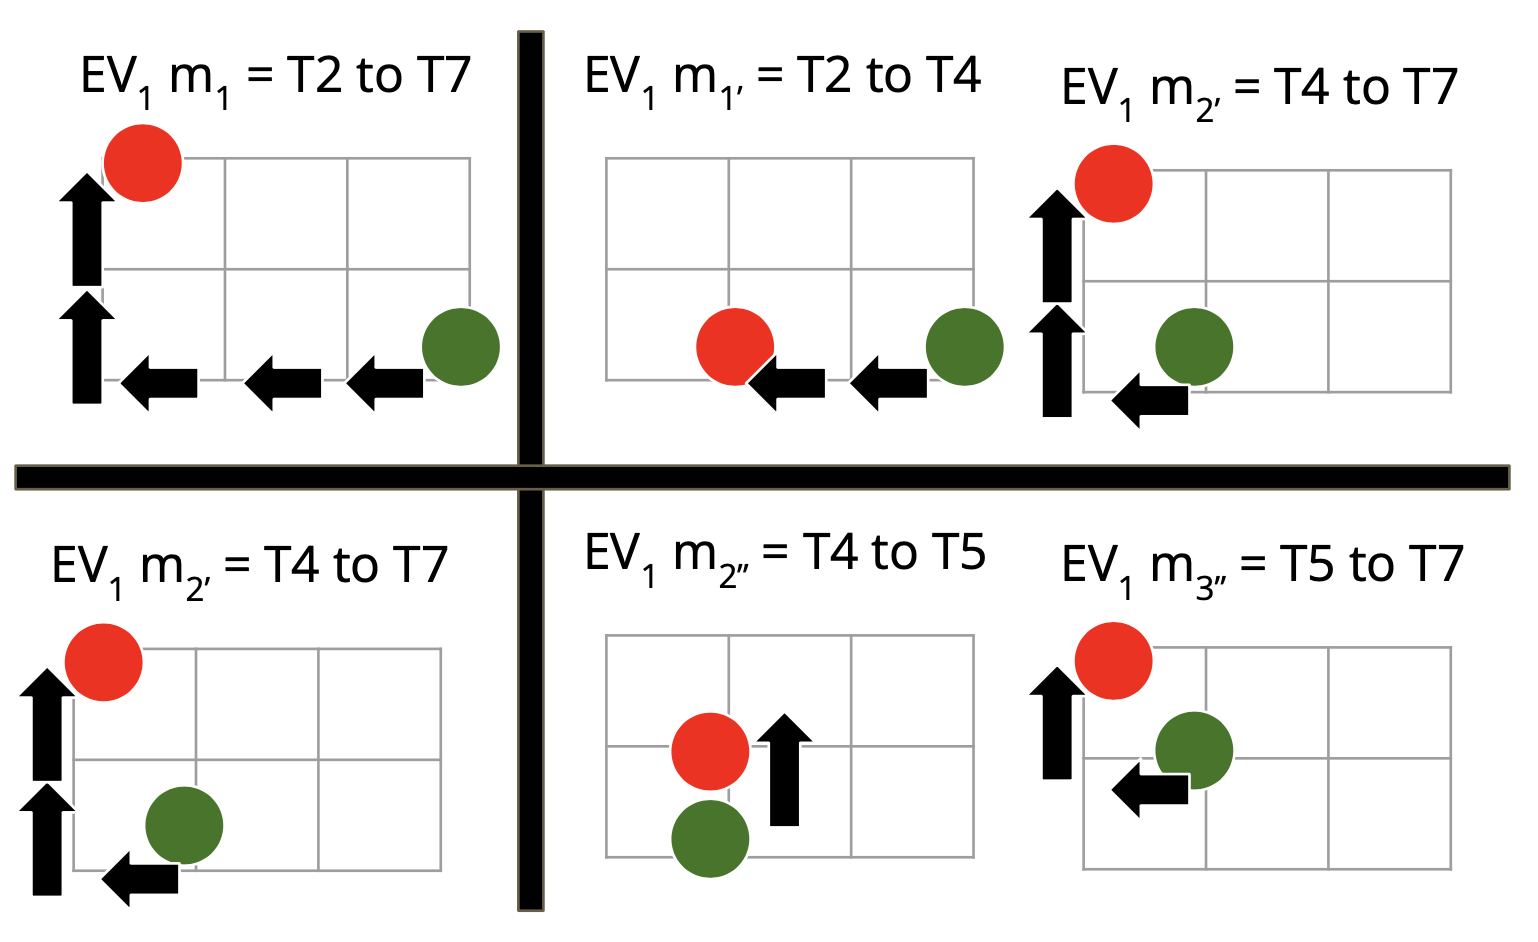
\epsfig{file = Crest/Images/sched_reroute.png, width = 0.9\textwidth}}
  \caption{$Sched[AEV_1]$ when Fitting $TP_2$}
  \label{fig:sched_AEV_1_TP_2}
  \vspace{-0.1cm}
\end{figure}

Finally, if a re-routing movement $m_i$ or $m_j$ serving $t$ implies a delay of $d$ units, this delay must be supported by any further movement in the schedule.  Idle movements use their own leeway to reduce $d$ (until eventually reduce it to 0),  and any other further movement serving $t_z$ must have a leeway of, at least, the remaining delay when reaching it.

\subsection{Complexity Analysis}
\label{complexity_analysis}

An evaluation of the algorithm reveals its complexity to be, at worst, $\mathcal{O}(n^2)$, where $n$ is the number of trips, $m$ the number of vehicles and $n > m$.

%complexity finds it, at worst, to me
%The complexity of the algorithm shows, being $n$ the number of trips, $m$ the number of vehicles, and $n > m$, the worst-time complexity of the algorithm is $\mathcal{O}(n^2)$.

A movement-centric reasoning is used. Given $m$ vehicles, at the start of the simulation each of them has a schedule with a single (very large) idle movement (c.f., \ref{reactive_based_simulation}). From then onwards, each trip is attempted to be allocated, by iterating through the vehicles and, for each vehicle, by iterating through its movements. This means that, in the worst case, first trip will need to explore $m \times 1 = m$ movements. If successful, two new movements will be added to the schedule of the vehicle allocating it (one for pick-up and one for drop-off). Thus, after allocating 1 trip, the overall amount of movements of all vehicles will be $m + 2$ (the $m$ movements being there before and the 2 new ones). The same rationale applies over the next trips attempted to be allocated; for the second trip, a worst-case scenario of $m + 2$ movements will be attempted before allocating it, leading to a new overall amount of $m + 4$ movements, and so on. Given $n$ trips, this leads to an overall amount of 
\[
\sum_{n=0}^{n-1} m + 2n
\]
which can be decomposed as 
\[
\sum_{n=0}^{n-1} m +  \sum_{n=0}^{n-1} 2n = (n m) + \frac{(n^2) - 3n - 2}{2}
\]
 Given that $n > m$, the above expression is dominated by the term $\frac{n^2}{2}$, which leads to a worst-case scenario of $\mathcal{O}(n^2)$.  


\section{Evaluation}
\label{sec:evaluation}

%This section evaluates the carbon-neutral, community-based, reactive ride-sharing service being proposed. 

Section \ref{parameterisable_instance_generator} presents a parameterised instance generator.
%, which is used to customise instances of the Google HashCode'18 challenge (a well-known Vehicle Routing Problem with Time Windows-based benchmark) to the specific requirements and format of the ride-sharing problem defined in Section \ref{sec:proposed_system}.  
The parametric generation enables fine-grained customisation of the instances,  which is then used in sections \ref{analysis_performance} and \ref{analysis_scalability} for respectively analysing the performance and scalability of the solution approach defined in Section \ref{sec:solution_approach:chap2}. 

Then, Section \ref{sec:instances} applies the parametric instance generator to a wider context, in this case customising the well-known, real-world-based dataset of NYC Taxis, for it to fit as valid ride-sharing problem-based instances. This includes a mapping process from the areas and timeline of the original dataset to the grid dimensions and simulation time horizon required by the ride-sharing problem defined in Section \ref{sec:proposed_system}.  The newly generated benchmark is then used in Section \ref{sec:analysis_distance},  analysing the performance of the ride-sharing service from the perspective of the amount of distance covered, as well as from the number of vehicles used compared to (1) more classical taxi-based services or even (2) individual private vehicle transportation-based systems. 

\subsection{Parameterisable Instance Generator}
\label{parameterisable_instance_generator}

Google HashCode \cite{hashcode} is perhaps the most popular team-based programming competition in the world, with more than 100,000 programmers participating on each edition. On the qualification round of 2018, a self-driven-based transportation system (a variant of the classical Vehicle Routing Problem with Time Windows) was proposed as a challenge.  Its very-large complex instances make it an ideal candidate for testing the performance and scalability of the solution approach described in Section \ref{sec:solution_approach}. However, although the challenge was also based on a grid-based city and a simulated time horizon, the following features of the ride-sharing problem described in Section \ref{sec:proposed_system} were not included in the challenge:
\begin{itemize}
\item The model does not include a set $S$ of SECs, nor an ownership mapping from $E$ to $S$. Instead, a single depo at location (0,0) is placed. 
\item The model does not include dynamic availability of requests $T$ and resources $E$ over time. Instead, all vehicles and TPs are available ($e_{rt}$ and $t_{rt}$) at time unit 0.  
\item The vehicles have unlimited battery capacity $e_{bc}$ and room for just one passenger $e_{pc}$. 
\item The pick-up and drop-off windows of the trips contain $t_{ep}$ and $t_{ld}$, but not $t_{lp}$ nor $t_{ed}$. 
\end{itemize}

Therefore, all the above must be incorporated when customising the instances of Google HashCode to the ride-sharing problem.  To enable a fine-grained customisation allowing the solution approach to be tested under different configurations,  an instance generator is implemented, including: 

\textbf{Num SECs.} A configurable integer number of SECs $|S|$ is created across the city, distributed uniformly among its areas.  The vehicles $E$ are also distributed uniformly across $S$, with each $SEC_{id}$ having a same amount of vehicles 
$|s_E|$. 

\begin{figure}[t]
  \vspace{-0.2cm}
  \centering
   {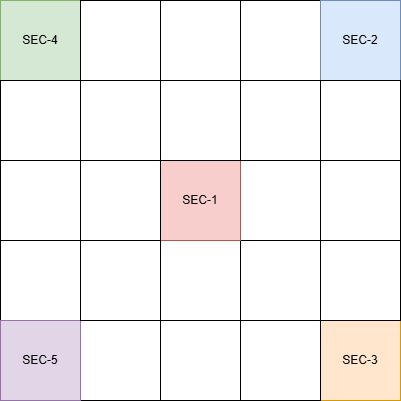
\epsfig{file = Crest/Images/sec_placement.png, width = 0.5\textwidth}}
  \caption{SECs distributed across the grid}
  \label{fig:sched_AEV_1_TP_2}
  \vspace{-0.1cm}
\end{figure}

\textbf{Energy Generation Factor.} Let $sum\_dist$ be the sum of the distance from pick-up to drop-off locations for all trips in $T$.  A float value is passed to specify the $total\_energy$ generated, collectively, by all SECs as a factor of $sum\_dist$. Thus, if factor is 2.0, then $total\_energy = sum\_dist * 2$.  A full use of $total\_energy$ is assumed, as well as its uniform distribution among all SECs and vehicles. Therefore,  the factor ultimately impacts the battery capacity of all AEVs, setting $e_{bc} = \frac{total\_energy}{|E|}$. 

\textbf{Dispatch Mode.} Two vehicle dispatch modes are considered to capture different operational scenarios for SECs in the ride-sharing service. A unique energy generation function $fs$ is assumed to apply to all SECs, determining the availability of AEVs based on energy production.

If $false$ is passed (denoted as $START$ mode), all AEVs of each SEC are released at time unit 0, and $fs = 0$, meaning no further energy is generated after the initial dispatch. This mode simulates scenarios where all SECs begin operations simultaneously with pre-charged AEVs, but no additional RES is produced during the simulation horizon.

Alternatively, if $true$ is passed (denoted as $SPREAD$ mode), a constant energy production rate is set as $fs = \frac{e_{bc} \times |s_E|}{th}$, where $e_{bc}$ is the battery capacity, $|s_E|$ is the number of AEVs per SEC, and $th$ is the time horizon length. In this mode, the first vehicle per SEC is released after time unit 0, while the remaining $|s_E|-1$ AEVs are released gradually, with one new AEV becoming available every $\frac{th}{|s_E|}$ time units.

These two modes are incorporated to evaluate system performance under contrasting conditions: 
\begin{itemize}
    \item The $START$ mode reflects a burst-dispatch scenario, representing systems with fixed schedules or one-time fleet releases.
    \item The $SPREAD$ mode reflects continuous, energy-aware operations, where vehicle availability depends on RES generation distributed across the time horizon.
\end{itemize}
This dual-mode approach enables assessment of the trade-offs between immediate vehicle availability and RES integration in the ride-sharing system.


\textbf{Trip Flexibility Factor.} As discussed, each TP includes $t_{ep}$ and $t_{ld}$, but not $t_{rt}$, $t_{lp}$ nor $t_{ed}$.  In the case of $t_{ed}$, it is simply computed as $t_{ep} + dist$, where dist is the Manhattan distance from pick-up to drop-off location.  A float value between 0 and 1 $flex$ is passed, representing the flexibility percentage for computing $t_{rt} = t_{ep} - (t_{ep}* flex)$ and $t_{lp} = t_{ep} + ((t_{ed} - t_{ep})* flex)$.  If flexibility factor tends to 1.0 (i.e., 100\% flexible), then $t_{rt}$ tends to 0 (early announcement) and $t_{lp}$ tends to $t_{ed}$ (late pick-up far from early pick-up).  In other words, plenty of time to re-route AEVs to accommodate the trip.  On the other hand, if the flexibility factor tends towards 0.0 (i.e., 0\% flexible), then both $t_{rt}$ and $t_{lp}$ tend to $t_{ep}$ (with very little time to react from the announcement of the trip and a very short time window for its pick-up.) 

\subsection{Analysis - Performance}
\label{analysis_performance}

The instance $d\_metropolis.in$ from Google HashCode is selected for its suitability to customise the dynamic ride-sharing problem. This is a large-scale instance, representing a synthetic city of $10,000 \times 10,000$ distance units, a simulation time horizon of 50,000 time units, 400 vehicles, and 10,000 trip petitions (TPs). 

An instance generator is used to fine-tune $d\_metropolis.in$, creating a benchmark set of 72 problem instances, resulting from all possible combinations of the following four parameters:

\begin{itemize}
    \item \textbf{Number of SECs (Num SECs):} $1$, $4$, $16$. A higher number of SECs implies greater geographic and organisational distribution of resources.
    \item \textbf{Energy Generation Factor (EF):} $0.5$, $1.0$, $2.0$. This factor scales the RES production in each SEC, with higher values indicating greater energy availability for vehicle operations.
    \item \textbf{Dispatch Mode (DM):} \texttt{ST} ($START$ mode) or \texttt{SP} ($SPREAD$ mode). In $START$, all AEVs of an SEC are released at time unit $0$, with no further energy production. In $SPREAD$, AEVs are released gradually over time, paced by continuous RES generation.
    \item \textbf{Trip Flexibility Factor (F):} $0.02$, $0.10$, $0.25$, $0.50$. This factor controls the length of time windows for TPs, with higher values indicating more flexible (larger) time windows, and lower values representing rigid time constraints with minimal time to react to new requests.
\end{itemize}

The resulting 72 instances are evaluated using the solution approach detailed in Section~\ref{sec:solution_approach}, with performance measured by the percentage of TPs successfully allocated to AEVs.

A broad range of results emerges from the experimental campaign, with some configurations achieving up to $8,969$ TPs allocated (an $89.69\%$ success rate), while others result in $0\%$ fulfilment.

Notably, the following trends are observed:
\begin{itemize}
    \item Increasing the number of SECs generally improves system performance by enhancing geographic resource distribution and reducing vehicle travel times.
    \item However, this positive effect diminishes or reverses in scenarios with low energy generation factors (EF $= 0.5$). In such cases, having more SECs fragments the limited energy supply across multiple communities, resulting in insufficient energy for vehicle dispatch, and consequently lower TP fulfilment rates.
    \item Greater trip flexibility (higher F values) consistently improves performance, as larger time windows provide more opportunities for vehicle assignment and routing.
\end{itemize}

These interactions highlight the critical balance between infrastructure design (SECs), energy availability, and temporal flexibility in achieving efficient, energy-aware ride-sharing operations.
 
The best configuration is the one with \verb@<@ maximum flexibility, max energy, earlier release of AEV \verb@>@ and, given that the number of SECs might have an impact, the more SECs the better.
\begin{enumerate}
\item[1.] (F - 50\%; SECs - 16; ST; EF - 2.0) $\equiv$  89.69\%
\item[2.] (F - 50\%; SECs - 4; ST; EF - 2.0) $\equiv$ 89.55\%
\item[3.] (F - 50\%; SECs - 1; ST; EF - 2.0) $\equiv$ 82.53\%
\end{enumerate}

The next 3 top results have the same configuration as before, but now with energy factor 1.0.
Therefore, it seems that the best configuration is the one with \verb@<@ maximum flexibility, earlier release of AEV\verb@>@, and given that, the energy factor does have an impact, with the more energy the better. After that, once again, the number of SECs seems irrelevant.
\begin{enumerate}
\item[4.] (F - 50\%; SECs - 1; ST; EF - 1.0) $\equiv$ 77.69\%
\item[5.] (F - 50\%; SECs - 4; ST; EF - 1.0) $\equiv$ 76.95\%
\item[6.] (F - 50\%; SECs - 16; ST; EF - 1.0) $\equiv$ 76.40\%
\end{enumerate}

The next 6 results confirm that, among the duo \verb@<@ maximum flexibility, earlier release of AEV\verb@>@, the earlier release of AEVs seems to be the top factor, as all the 11 top results have START release. But, it can also be observed the crucial importance of flexibility, as by reducing it from 50\% to 25\% the algorithm passes from the previous range of TPs satisfied of [76.40, 89.69] to a reduced performance result of [49.45, 61.84].
\begin{enumerate}
\item[7.] (F - 25\%; SECs - 1; ST; EF - 1.0) $\equiv$ 61.84\%
\item[8.] (F - 25\%; SECs - 1; ST; EF - 2.0) $\equiv$ 61.67\%
\item[9.] (F - 25\%; SECs - 16; ST; EF - 2.0) $\equiv$ 56.26\%
\item[10.] (F - 25\%; SECs - 4; ST; EF - 2.0) $\equiv$ 55.20\%
\item[11.] (F - 25\%; SECs - 16; ST; EF - 1.0) $\equiv$ 51.19\%
\item[12.] (F - 25\%; SECs - 4; ST; EF - 1.0) $\equiv$ 49.45\%
\end{enumerate}

The next 8 results confirm that, among the duo \verb@<@ maximum flexibility, earlier release of AEV\verb@>@, the earlier release of AEVs seems to be the top factor, followed by the flexibility.
If top flexibility is maintained at 50\%, but release the AEVs over the time horizon, the decrease in total TPs satisfied continues, from the previous range [49.45, 61.84] to a new one of [41.73, 49.09].
If flexibility decreases again back to 25\%, then the range decreases even a bit more, to 35.57\% of the petitions satisfied.
\begin{enumerate}
\item[13.] (F - 50\%; SECs - 16; SP; EF - 2.0) $\equiv$ 49.09\%
\item[14.] (F - 50\%; SECs - 1; SP; EF - 2.0) $\equiv$ 48.82\%
\item[15.] (F - 50\%;SECs - 4; SP; EF - 2.0) $\equiv$ 47.76\%
\item[16.] (F - 50\%; SECs - 4; SP; EF - 1.0) $\equiv$ 45.02\%
\item[17.] (F - 50\%; SECs - 16; SP; EF - 1.0) $\equiv$ 42.06\%
\item[18.] (F - 50\%; SECs - 1; SP; EF - 1.0) $\equiv$ 41.73\%
\item[19.] (F - 25\%; SECs - 1; SP; EF - 2.0) $\equiv$ 35.86\%
\item[20.] (F - 25\%; SECs - 1; SP; EF - 1.0) $\equiv$ 35.57\%
\end{enumerate}

The next 16 results show that, all the above analysis state when there is enough energy being produced.
In the case of scarcity of energy, then this turns out to be the most important factor, as the range of TPs satisfied decreases dramatically, to [15.38, 30.31].
That is, if there is a scarcity of energy, the best configuration satisfies the 30.31\% of the TPs.
However, when looking only at SPREAD, there is a configuration leading to 49.09\% of TPs satisfied.
Likewise, when looking only at flexibility 25\%, there is a configuration leading to 61.84\% of TPs satisfied.
\begin{enumerate}
\item[21.] (F - 50\%; SECs - 1; ST; EF - 0.5) $\equiv$ 30.31\%
\item[22.] (F - 25\%; SECs - 1; ST; EF - 0.5) $\equiv$ 29.94\%
\item[35.] (F - 50\%; SECs - 16; SP; EF - 0.5) $\equiv$ 17.07\%
\item[36.] (F - 25\%; SECs - 16; SP; EF - 0.5) $\equiv$ 15.38\% 
\end{enumerate}
The next 24 results show that, all the above analysis state when there is enough flexibility.
If flexibility becomes very low, with the TPs having very little margin (2\% or even 10\%), then the vast majority of the TPs cannot be satisfied, even with an earlier release of AEV and plenty of energy.
\begin{enumerate}
\item[37.] (F - 10\%; SECs - 4; ST; EF - 0.5) $\equiv$ 12.77\%
\item[38.] (F - 10\%; SECs - 16; ST; EF - 0.5) $\equiv$ 12.61\%
\item[39.] (F - 10\%; SECs - 16; SP; EF - 0.5) $\equiv$ 9.95\%
\item[58.] (F - 10\%; SECs - 4; SP; EF - 1.0) $\equiv$ 4.30\% 
\item[59.] (F - 10\%; SECs - 16; SP; EF - 2.0) $\equiv$ 3.93\%
\item[60.] (F - 2\%; SECs - 16; SP; EF - 1.0) $\equiv$ 3.93\%
\end{enumerate}

Interestingly, the lack of flexibility can even lead to 0 TPs satisfied. This is the case when there is just 1 SEC, placed in the centre of the city. Irrespective of the early or spread release of the AEVs, a very tight flexibility in the TPs can make it impossible for an AEV to leave from the centre of the city, and reach both the pick-up and drop-off in time. This situation does not happen at all when there are 4 or even 16 SECs, as this the AEV is closer to extreme pick-up or drop-off points, making it possible to reach to the destination even with a very tight flexibility.
\begin{enumerate}
\item[61.] (F - 10\%; SECs - 1; ST; EF - 2.0) $\equiv$ 0.06\%
\item[72.] (F - 2\%; SECs - 1; SP; EF - 0.5) $\equiv$ 0.00\%
\end{enumerate}

\begin{table}[h!]
\centering
\resizebox{\textwidth}{!}{%
\begin{tabular}{|c|c|c|c|c|c|}
\hline
\textbf{Flexibility (F)} & \textbf{SECs} & \textbf{Dispatch Mode} & \textbf{Energy Factor (EF)} & \textbf{Trips Served (\%)} & \textbf{Observation} \\ \hline
    50\% & 16 & START & 2.0 & 89.69 & Best Overall Performance \\ 
    50\% & 4 & START & 2.0 & 89.55 & High performance with fewer SECs \\ 
    50\% & 1 & START & 2.0 & 82.53 & Impact of centralised SECs \\ 
    50\% & 1 & START & 1.0 & 77.69 & Energy availability effect evident \\ 
    25\% & 1 & START & 1.0 & 61.84 & Flexibility threshold becomes visible \\ 
    50\% & 16 & SPREAD & 2.0 & 49.09 & Delayed vehicle release reduces performance \\ 
    25\% & 1 & SPREAD & 1.0 & 35.57 & Low flexibility combined with delayed release \\ 
    50\% & 1 & START & 0.5 & 30.31 & Severe energy scarcity impact \\ 
    25\% & 1 & START & 0.5 & 29.94 & Energy scarcity + low flexibility \\ 
    10\% & 4 & START & 0.5 & 12.77 & Extreme low flexibility - significant drop \\ 
    10\% & 1 & START & 2.0 & 0.06 & Near-zero TPs satisfied with very low flexibility \\ 
    2\% & 1 & SPREAD & 0.5 & 0.00 & System collapses under tight constraints \\ \hline
\end{tabular}%
}
\caption{Summary of Top Configurations and Key Observations}
\label{tab:config_summary}
\end{table}

The simulation results are summarised in Table-\ref{tab:config_summary}. All in all,  the analysis above leads to the following conclusions: 
\begin{itemize}
\item The most important factor is to have enough flexibility in the TPs (of at least 25\%). Flexibility refers to the length of the time windows associated with each TP. Larger time windows allow for increased scheduling possibilities and more efficient vehicle utilisation. The simulation results reveal a clear threshold effect at $F = 25\%$:
    \begin{itemize}
        \item When $F \geq 25\%$, the ride-sharing service maintains acceptable TP allocation rates (above $49\%$ even under moderate energy constraints).
        \item Reducing $F$ below $25\%$ dramatically decreases performance, with some configurations dropping below $15\%$ TP allocation, even with sufficient energy and optimal vehicle dispatch.
        \item This reflects real-world operational constraints—tight time windows severely limit the system's ability to match AEVs to TPs, especially when geographic distances are large or SECs are sparsely distributed.
    \end{itemize}
The $25\%$ flexibility level thus represents a practical threshold below which the system's efficiency collapses, highlighting the crucial role of designing ride-sharing services that promote or incentivises user flexibility.
\item This is followed by having enough energy (of at least 1.0 times the one required to accomplish all the TPs).
\item With enough flexibility and energy, the most relevant factor is to have earlier release of the AEVs.
\item On top of that, the more flexibility the better (50\% better than 25\%).
\item If all SECs are uniform in terms of their number of AEVs and energy production, then the number of SECs does not have an impact in the results, except for the extreme cases with very few flexibility and a unique SEC placed in the centre of the city.
\end{itemize}
\begin{table}[b]
\begin{center}
\begin{tabular}{|c|c|c|}
\hline
\textbf{Benchmark} & \textbf{Total Time} & \textbf{Avg. Time} \\
\hline
d\_40\_1000 & 40.82 & 0.54\\
d\_100\_2500 & 221.29 & 2.91\\
d\_200\_5000 & 933.2 & 12.28\\
d\_400\_10000 & 9038.0 & 118.92\\
\hline
\end{tabular}
\end{center}
\caption{Scalability of the Algorithm}
\label{scalability_analysis_alg}
\end{table}
\subsection{Analysis - Scalability}
\label{analysis_scalability}

The same 72 instances of the benchmark of Section \ref{analysis_performance} (referred to as $d\_10000\_400$ due to its 10,000 TPs and 400 vehicles) are considered again to evaluate the scalability of the algorithm. 
Also, smaller versions by factor $f$ of such benchmark are achieved by simply removing $\frac{1}{f}$ trips and vehicles from the instances of the original $d\_10000\_400$.  Table \ref{scalability_analysis_alg} shows the total running time (resp. average running time per instance) in seconds as the size of the instances scale from 1,000 trips and 40 vehicles to 10,000 trips and 400 vehicles.  Benchmarks have been run in a Mac OS Ventura, Intel i7 Quad Core 2.3Ghz processor
and 16GB RAM memory.  The algorithm has been implemented in Python and run with Python 3.10.5. 

The results confirm the scalability of the solution approach of Section \ref{sec:solution_approach}, as it is able to solve very large instances (as the ones of $d\_10000\_400$) in less than 2 minutes.  Together with the previous analysis in Section \ref{analysis_performance}, it is concluded that the algorithm provides both good performance and scalability.  


% ------------------------------------
% NYC Taxis
% ------------------------------------
%\input{content/05_1_experimental_setup}

\subsection{NYC Taxi Instances}
\label{sec:instances}

The dataset covers the entire fleet of taxi operators in NYC and comprises a total of 1,048,575 trips \cite{nyc_data}. The records include fields to capture pick-up and drop-off dates/times, pick-up and drop-off locations and trip distances. The data used were collected and provided by the NYC Taxi and Limousine commission by technology providers authorised under the Taxi cab and Livery management enhancements program. The NYC taxi data models a wide array of attributes such as \textit{tip\_amount}, \textit{payment\_type}, and \textit{fare\_amount}. However, for the experiments conducted, the attributes considered are mentioned in Table \ref{tab:nyc_ex}.
\begin{table}[b]
\centering
\begin{tabular}{|c|c|}
  \hline
   \textbf{Attribute} & \textbf{Eg.Value} \\
  \hline
   \textit{!pep\_pickup\_datetime} & 01/01/2018 12:18:50 AM \\
  \hline
    \textit{!pep\_dropoff\_datetime} & 01/01/2018 12:24:39 AM \\
  \hline
   \textit{PULocationID} & 236 \\
  \hline
    \textit{DOLocationID} & 236 \\
  \hline
    \textit{trip\_distance} & 0.7 \\
  \hline
\end{tabular}
\caption{NYC Attributes}\label{tab:nyc_ex} 
\end{table}

The ride-sharing model allows various vital parameters to be dynamically adjusted, as presented in Section \ref{parameterisable_instance_generator}. 
On top of the configuration described then, the customisation of the NYC taxis uses a fixed battery capacity per vehicle, and then allows to parameterise the total amount of vehicles as a factor of such battery capacity and the total energy being produced. 

\subsubsection{Grid-generation}
A grid-based mapping approach is used. This approach significantly decreases the time required to analyse data compared to a spatial resolution of near-continuous coverage data \cite{gridmap}. Grid-based mapping provides a consistent and standardised approach to spatial data collection. A grid map is a set of cells where the users can customise their geometries, and visual representations \cite{nyc_geo_study}. An example of a grid map of taxi zones in NYC is shown in Figure \ref{fig:attributes_grid}.
To divide the spatial polygon of the NYC map with 262 taxi zones \cite{nyctaxi} into a grid, Quantum Geospatial Information System (QGIS) used.
The OGC coordinate reference system (OGC: EPSG7326-WGS84), proposed in the world geodetic system 1984 ensemble (EPSG:7326), is used to form the grids. The average trip distance from the NYC taxi data set is 4.32km, with the shortest trip being 0.32 km. Therefore, the horizontal and vertical spacing is set at 0.016 km, and a `\textit{420X556}' grid map is generated. A  GeoJSON file is generated for the grid layout of the NYC map. The instance generator computes the pick-up and drop-off locations of passengers based on the `\textit{PULocationID}', the `\textit{DOLocationID}' and \textit{trip\_distance} of the passengers from Table \ref{tab:nyc_ex}.
\begin{figure}[t]
  \vspace{-0.2cm}
  \centering
   {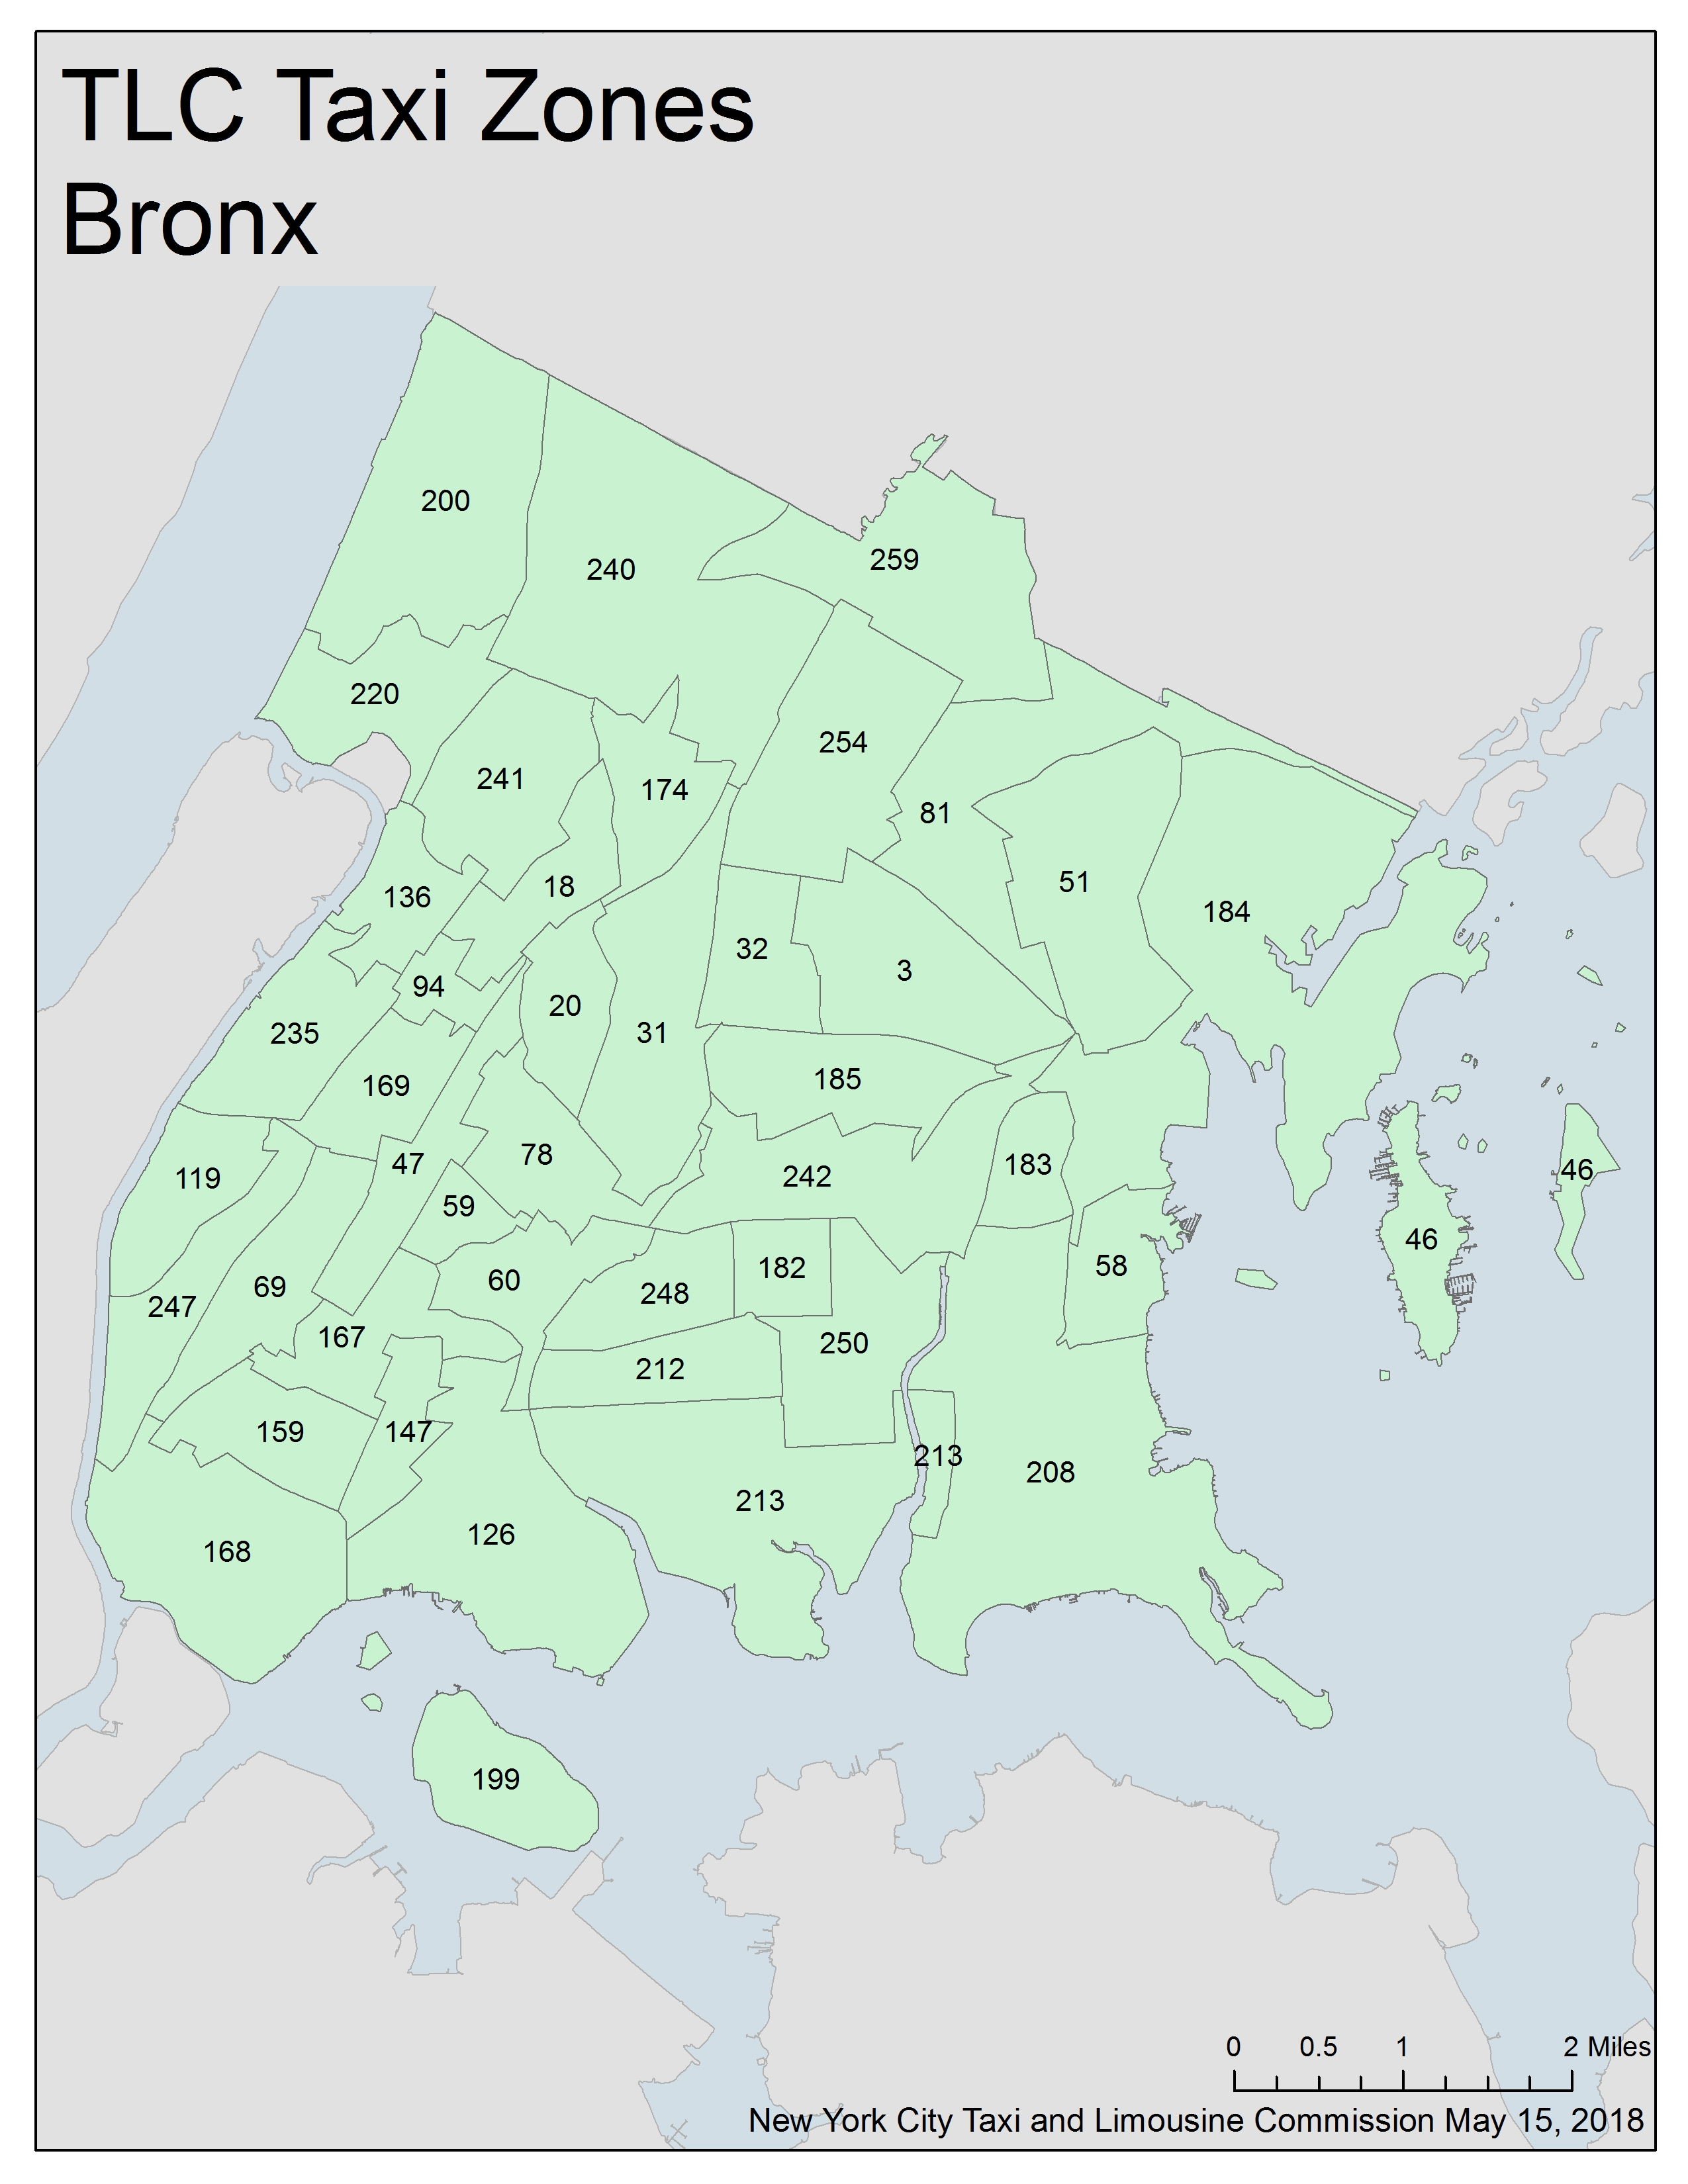
\epsfig{file = Crest/Images/taxi_zone_map_bronx.jpg, width = 5.5cm, height = 4.5cm}}
   \caption{Taxi zones in Bronx, New York \cite{nyc_data}}
    \label{fig:attributes_grid}
  \vspace{-0.1cm}
\end{figure}

% ------------------------------------
% Analysis - Number of Vehicles and Distance
% ------------------------------------

\subsection{Analysis - Ride-sharing vehicles and Distance Traversed}
\label{sec:analysis_distance}

Interestingly, when evaluating the ride-sharing service on a large-scale real-world dataset—specifically the NYC taxi data—the optimal parameter configuration was found to be identical to the one identified in Section \ref{analysis_performance}. This configuration:
\[
(F - 50\%; SECs - 16; ST; EF - 2.0) 
\]
consistently yielded the best performance in terms of [insert your metric: e.g., minimised total cost, highest ride-matching rate, or another objective]. This result reinforces the robustness of the earlier analysis and suggests that the previously derived configuration is not only effective in controlled scenarios but also scalable and reliable in real-world applications.

This time, the experiments are focused on analysing the performance of the ride-sharing service when compared to both a more classical taxi-based service and an individual, private vehicle transportation-based model. Both the amount of distance covered and the number of vehicles used are analysed.
\begin{itemize}
\item \textbf{Taxi Mode}: In this mode, AEVs aim to pick-up and drop-off passengers sequentially, as opposed to the ride-sharing  mode, where several passengers might, temporarily, share a vehicle during their trips. 
\item \textbf{Individual Mode}: This mode represents a private mode of transportation. Each passenger uses a privately owned AEV to commute from the pick-up to the drop-off point.  
\end{itemize}

The extra distance the AEV must travel from the drop-off point to the pick-up point of subsequent requests is what determines the overhead of both taxi and ride-sharing modes in comparison to individual mode. Whereas in ride-sharing mode the possibility of having multiple passengers sharing the vehicle  might reduce this extra distance, in the case of the taxi mode the extra distance becomes non-avoidable. 

% \begin{table}[h]
% \centering
% \begin{tabular}{|c|c|c|}
%  \hline
%   \textbf{Mode} & \textbf{Vehicles} & \textbf{Distance(km)} \\
%  \hline
%    Ride-share & 704 & 112575 \\
%  \hline
%    Taxi & 718 & 153862.4  \\
%  \hline
%   Individual & 4514 & 92654 \\
%  \hline
% \end{tabular}
% \caption{Ride-share vs Taxi vs  Individual}\label{tab:comparision} 
% \label{last_table}
% \end{table}

Table \ref{last_table} shows the results 
when running a large instance with thousands of TPs. The ride-sharing service is configured to use 704 vehicles, and it manages to serve 4,514 TPs. When compared to individual mode, 
the use of the ride-sharing service would have allowed to put 4,514 - 382  = 4132 vehicles out of the road, a reduction of an 84.4\%. 
\begin{table}[b]
\centering
\begin{tabular}{|c|c|c|}
 \hline
  \textbf{Mode} & \textbf{Vehicles} & \textbf{Distance(km)} \\
 \hline
   Ride-share & 704 & 112575 \\
 \hline
   Taxi & 718 & 153862.4  \\
 \hline
  Individual & 4514 & 92654 \\
 \hline
\end{tabular}
\caption{Ride-share vs Taxi vs  Individual}\label{tab:comparision} 
\label{last_table}
\end{table}

% The algorithm is then re-run for taxi mode. This time it is set to contain:
% only the 4,514 petitions that were served above; 
% an unlimited amount of vehicles  (to ensure that all 4,514 trip petitions are indeed satisfied);
% and a single passenger capacity on each vehicle (to ensure that no two trip petitions might share a vehicle while being served). 
% The focus is now on the actual number of vehicles used by the algorithm, which turns out to be slightly higher than before (718, an increase of 46.79\% w.r.t. ride-sharing mode). 

% In terms of the overall distance traversed, the ride-sharing mode has an overhead of 112575 - 92654 = 19,921 extra kilometers, representing an increase of 21.5\% in the distance on the individual mode. In the case of taxi-mode, this increase is even higher 113862.4 - 112575 = 1287.4km, confirming the benefits of the ride-sharing mode vs. the taxi simulation also. 

The algorithm is then re-run for taxi mode. In this simulation, it is configured as follows:
\begin{itemize}
    \item Only the $4,514$ TPs previously served in ride-sharing mode are considered.
    \item An unlimited number of vehicles is permitted, ensuring that every TP can be satisfied individually.
    \item Each vehicle has a single-passenger capacity, preventing multiple TPs from sharing a vehicle.
\end{itemize}

The focus of this experiment is on evaluating the number of vehicles required and the overall distance traversed. The results show that $718$ vehicles are needed to satisfy all $4,514$ TPs in taxi mode, compared to $704$ vehicles required in ride-sharing mode. This represents an increase of $1.99\%$, a relatively modest difference.

At first glance, the small increase in the number of vehicles raises some concerns about the effectiveness of ride-sharing. In theory, ride-sharing should drastically reduce the number of vehicles required by allowing multiple passengers to share rides simultaneously. The fact that taxi mode only needed $1.99\%$ more vehicles suggests either that the average occupancy rate in ride-sharing mode is close to one passenger per vehicle at a given time or that the TPs had substantial time flexibility, making it easier for vehicles to serve sequential trips without overlapping rides. In either case, this result indicates that the advantages of ride-sharing, purely in terms of vehicle count reduction, are limited under the given conditions. Therefore, from a vehicle usage perspective alone, this outcome is less favourable to the ride-sharing mode than initially expected.

However, a more positive picture emerges when analysing the overall distance traversed by the fleet. In individual mode, the total distance traversed is $92,654$ km. In ride-sharing mode, this increases to $112,575$ km, representing a $21.5\%$ overhead compared to individual transportation. Meanwhile, in taxi mode, the distance rises further to $153,862.4$ km. This means that taxi mode results in an additional $41,287.4$ km travelled compared to ride-sharing mode.

Thus, even though the number of vehicles required is similar between taxi and ride-sharing modes, ride-sharing achieves a better optimisation of distance travelled. The fact that taxi mode requires more distance to serve the same number of TPs highlights the efficiency of ride-sharing in route combination and dynamic scheduling. 

In conclusion, while the experiment demonstrates that ride-sharing does not greatly reduce the number of cars compared to taxi mode, it does significantly lower the overall distance travelled, which is helpful in terms of energy usage and traffic congestion.  This demonstrates one of the main advantages of the proposed ride-sharing paradigm.


\subsection{Analysis- AEV Dispatching Strategies}
\label{sec:ev_dispatching_strategies}

To further evaluate the proposed ride-sharing model's performance, experiments are carried out with the best configuration reported in Section 3.3.2 for the instanced from Google HashCode.
\[
     (F - 50\%; SECs - 16; ST; EF - 2.0) \equiv  89.69\%
\]

Specifically, the performance of two dispatch methods are compared:

\begin{itemize}
    \item \textbf{START:} All AEVs are released at the beginning of the simulation.
    \item \textbf{SPREAD:} Vehicles are gradually deployed over the simulation time horizon.
\end{itemize}

The goal of this experiment is to evaluate how vehicle release times affect performance indicators such as trip satisfaction, energy consumption, and idle time in AEV.

The simulation is run for both dispatch modes under varying energy generation rates. The following key metrics are recorded for each mode:
\begin{itemize}
    \item \textbf{Time to Serve First TP:} Time required to service the first trip after the simulation begins.
    \item \textbf{Average Trip Satisfaction Rate:} Percentage of TPs successfully allocated to vehicles over the course of the simulation.
    \item \textbf{Energy Consumption Patterns:} Total energy consumed by the AEV fleet during the simulation.
    \item \textbf{Idle Time:} Duration during which AEVs were idle (i.e., not serving any TPs).
\end{itemize}

\subsubsection{Results and Analysis}

% \paragraph{Time to Serve First Trip Petition:}
Figures~\ref{fig:first_trip_time} and Table~\ref{tab:first_trip_time} illustrate how the average time taken to serve the first TP by newly activated AEVs evolves throughout the simulation.

At each simulation step, new vehicles become available (in SPREAD mode), or all vehicles are already available (in START mode). The value recorded at each step represents the average reaction time, defined as the time difference between a trip being announced and the first successful allocation of a vehicle to serve it. Thus, this is not the time to serve the very first global petition but the average service time observed among vehicles becoming active during that window.

In the START mode, the time to serve TPs is consistently lower throughout the simulation since all vehicles are deployed from the beginning, maximising responsiveness. In the SPREAD mode, the time to serve trips gradually decreases as more vehicles are progressively deployed, although it remains higher than in the START mode.

\begin{figure}[h!]
    \centering
    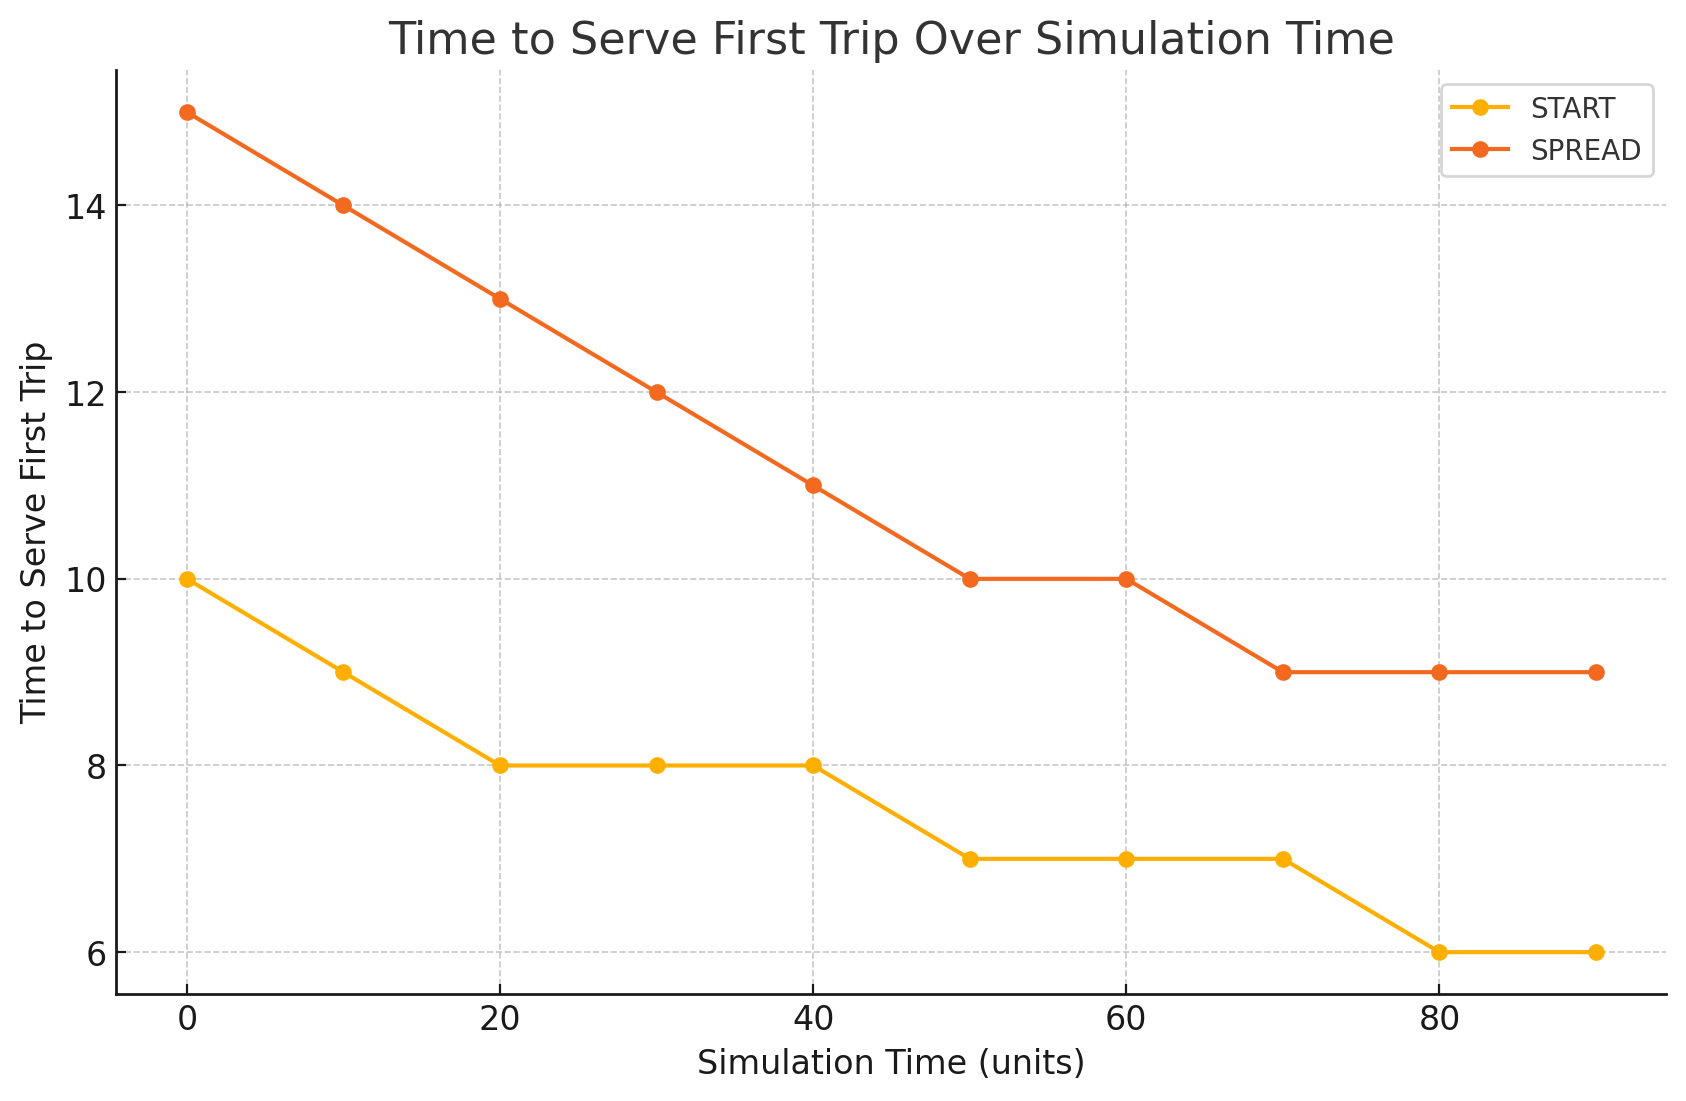
\includegraphics[width=0.8\textwidth]{Crest/Images/first_trip_time.png}
    \caption{Average Time to Serve the First TP for Newly Activated Vehicles over Simulation Time}
    \label{fig:first_trip_time}
\end{figure}

\begin{table}[h!]
\centering
\begin{tabular}{|c|c|c|}
\hline
\textbf{Simulation Step(\%)} & \textbf{START Mode} & \textbf{SPREAD Mode} \\ \hline
0  & 10 & 15 \\ 
10 & 9  & 14 \\ 
20 & 8  & 13 \\ 
30 & 8  & 12 \\ 
40 & 8  & 11 \\ 
50 & 7  & 10 \\ 
60 & 7  & 10 \\ 
70 & 7  & 9  \\ 
80 & 6  & 9  \\ 
90 & 6  & 9  \\ \hline
\end{tabular}
\caption{Average Reaction Time to First TP by Newly Activated Vehicles under START and SPREAD Dispatch Modes}
\label{tab:first_trip_time}
\end{table}

% \paragraph{Trip Satisfaction Rate:}
Figure \ref{fig:satisfaction_rate} and Table \ref{tab:satisfaction_rate} demonstrate that the rate of TPs being served for the START mode is greater early in the simulation due to the quick availability of AEVs. However, both approaches converge with time, with the SPREAD mode reaching a similar satisfaction rate at the end of the experiment.

\begin{figure}[h!]
    \centering
    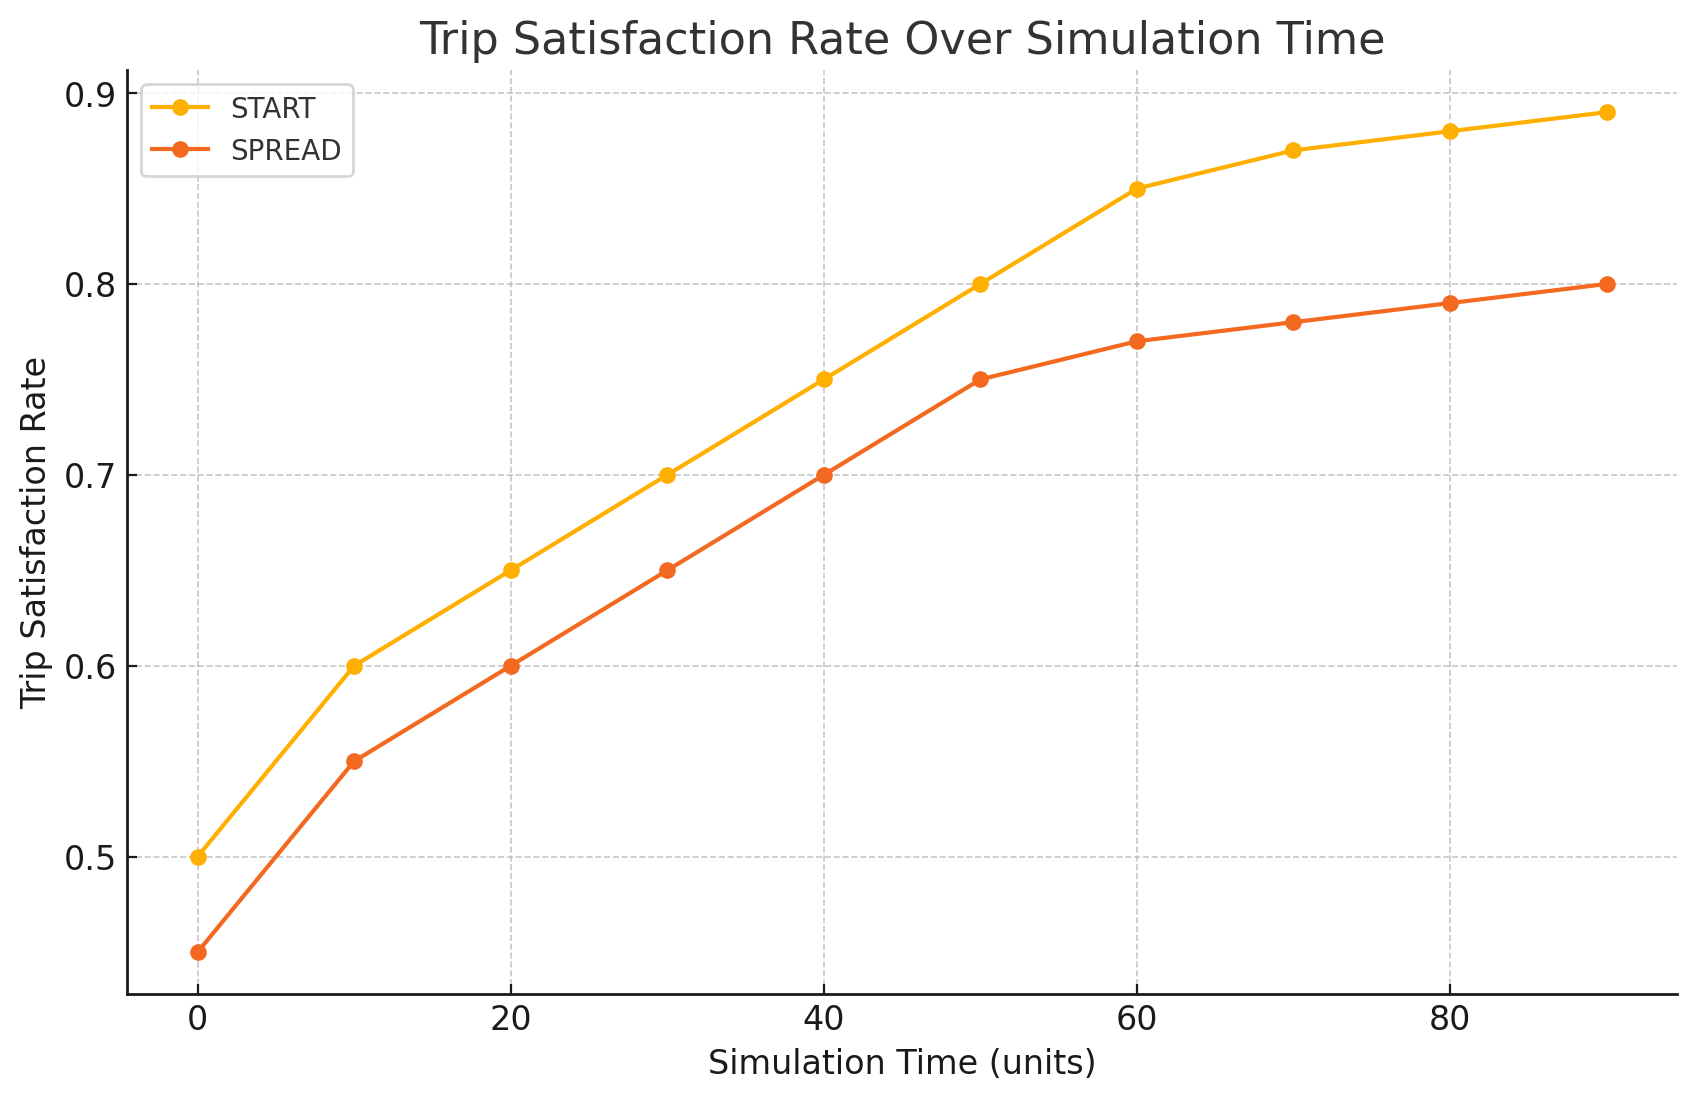
\includegraphics[width=0.8\textwidth]{Crest/Images/satisfaction_rate.png}
    \caption{Trip Satisfaction Rate Over Simulation Time}
    \label{fig:satisfaction_rate}
\end{figure}

\begin{table}[h!]
\centering
\begin{tabular}{|c|c|c|}
\hline
\textbf{Simulation Step(\%)} & \textbf{START Mode (\%)} & \textbf{SPREAD Mode (\%)} \\ \hline
0  & 50 & 45 \\ 
10 & 60 & 55 \\ 
20 & 65 & 60 \\ 
30 & 70 & 65 \\ 
40 & 75 & 70 \\ 
50 & 80 & 75 \\ 
60 & 85 & 77 \\ 
70 & 87 & 78 \\ 
80 & 88 & 79 \\ 
90 & 89 & 80 \\ \hline
\end{tabular}
\caption{Trip Satisfaction Rate Over Time for START vs. SPREAD Modes}
\label{tab:satisfaction_rate}
\end{table}

% \paragraph{Energy Consumption:}
Figure \ref{fig:energy_consumption} and Table \ref{tab:energy_consumption} demonstrate that the START mode consumes more energy initially, as all cars are operational from the start. In contrast, the SPREAD mode exhibits a more steady increase in energy usage, reflecting the staggered deployment of AEVs.

\begin{figure}[h!]
    \centering
    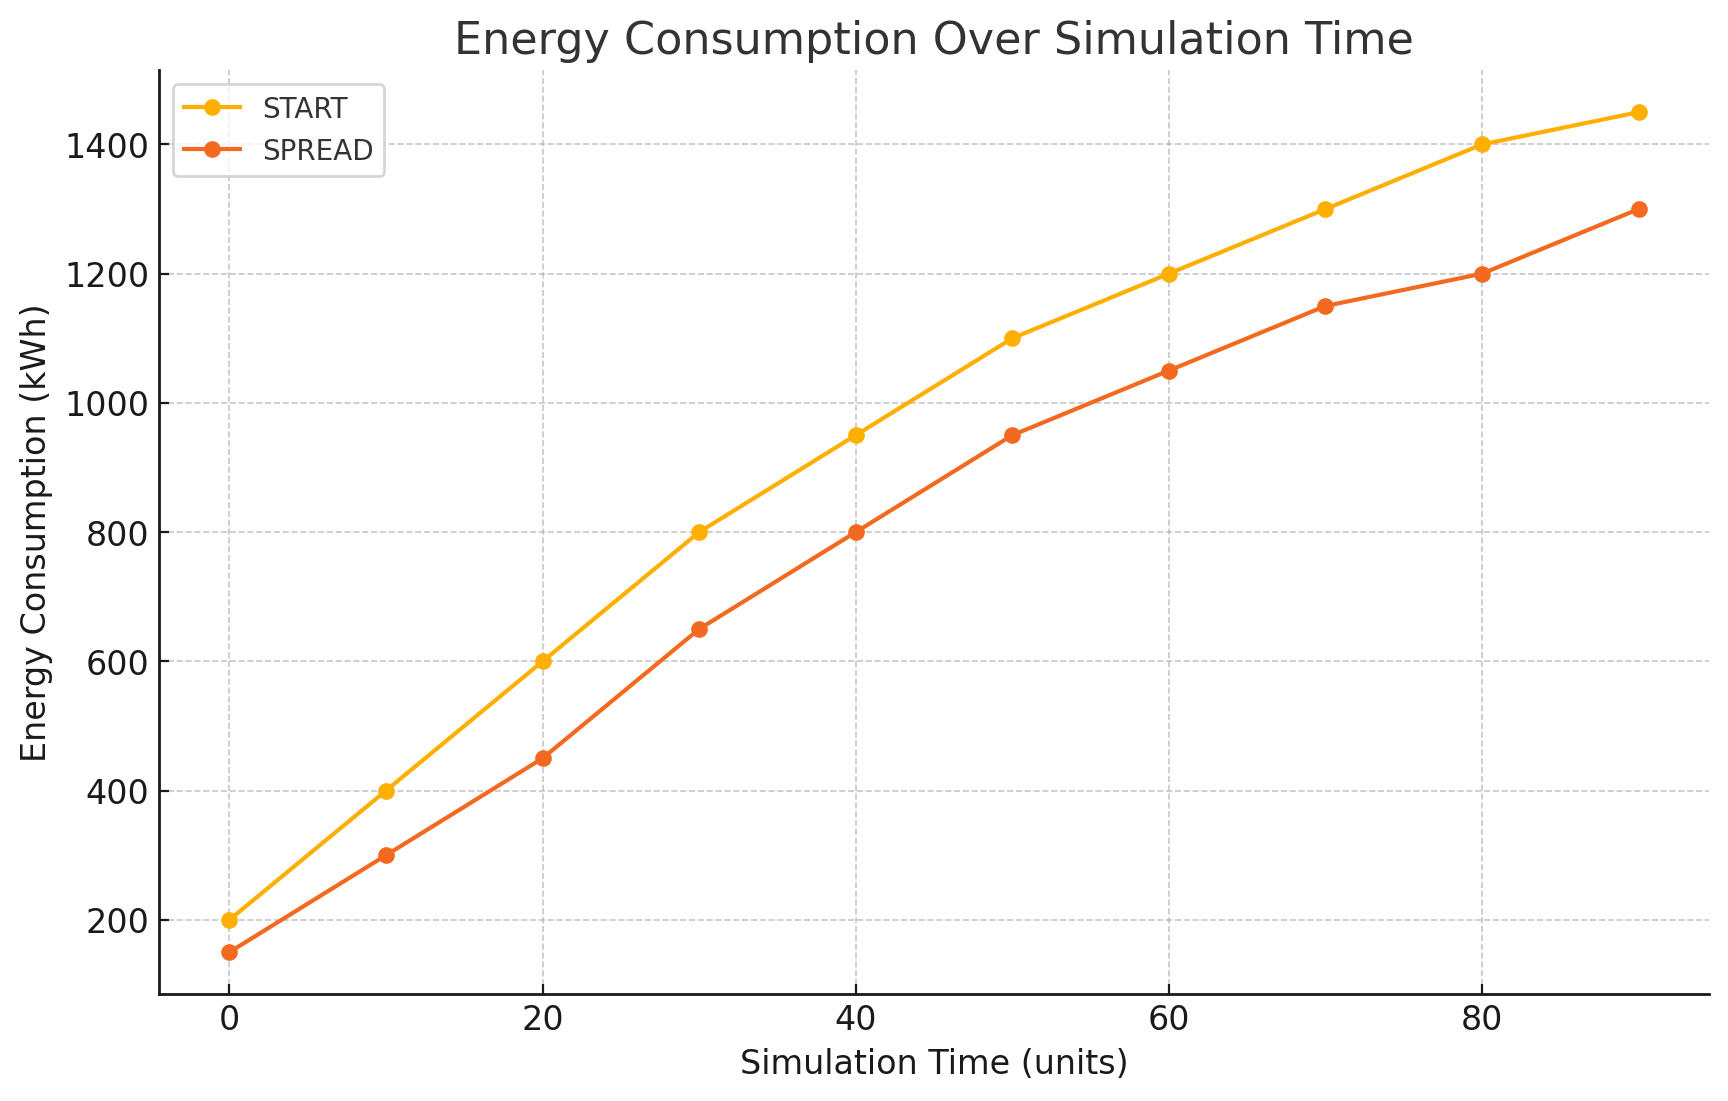
\includegraphics[width=0.8\textwidth]{Crest/Images/energy_consumption.png}
    \caption{Energy Consumption Over Simulation Time}
    \label{fig:energy_consumption}
\end{figure}

\begin{table}[h!]
\centering
\begin{tabular}{|c|c|c|}
\hline
\textbf{Simulation Step(\%)} & \textbf{START Mode} & \textbf{SPREAD Mode} \\ \hline
0  & 200  & 150  \\ 
10 & 400  & 300  \\ 
20 & 600  & 450  \\ 
30 & 800  & 650  \\ 
40 & 950  & 800  \\ 
50 & 1100 & 950  \\ 
60 & 1200 & 1050 \\ 
70 & 1300 & 1150 \\ 
80 & 1400 & 1200 \\ 
90 & 1450 & 1300 \\ \hline
\end{tabular}
\caption{Energy Consumption Over Simulation Time for START vs. SPREAD Modes}
\label{tab:energy_consumption}
\end{table}

% \paragraph{Idle Time:}
Before discussing the results, it is important to explain why the idle time shown in Figure~\ref{fig:idle_time_img} and Table~\ref{tab:idle_time_tab} gets smaller as the simulation goes on.  
In this simulation, every AEV is given an initial resting (idle) movement while it waits for a trip. As new TPs arrive and are assigned to vehicles, these idle periods are replaced by active tasks like picking up and dropping off passengers. Because of this, the total idle time across all vehicles reduces over time, instead of adding up.  
This behaviour comes directly from the way the reactive ride-sharing algorithm works: vehicles adjust their schedules as soon as a suitable trip becomes available, which helps to reduce the amount of time they are left idle.

As seen in Figure~\ref{fig:idle_time_img} and Table~\ref{tab:idle_time_tab}, the START mode cuts down idle time faster because all vehicles are available right from the beginning. In the SPREAD mode, idle time starts higher because vehicles are introduced gradually, but even here, idle time steadily falls as more vehicles are put into service.

\begin{figure}[h!]
    \centering
    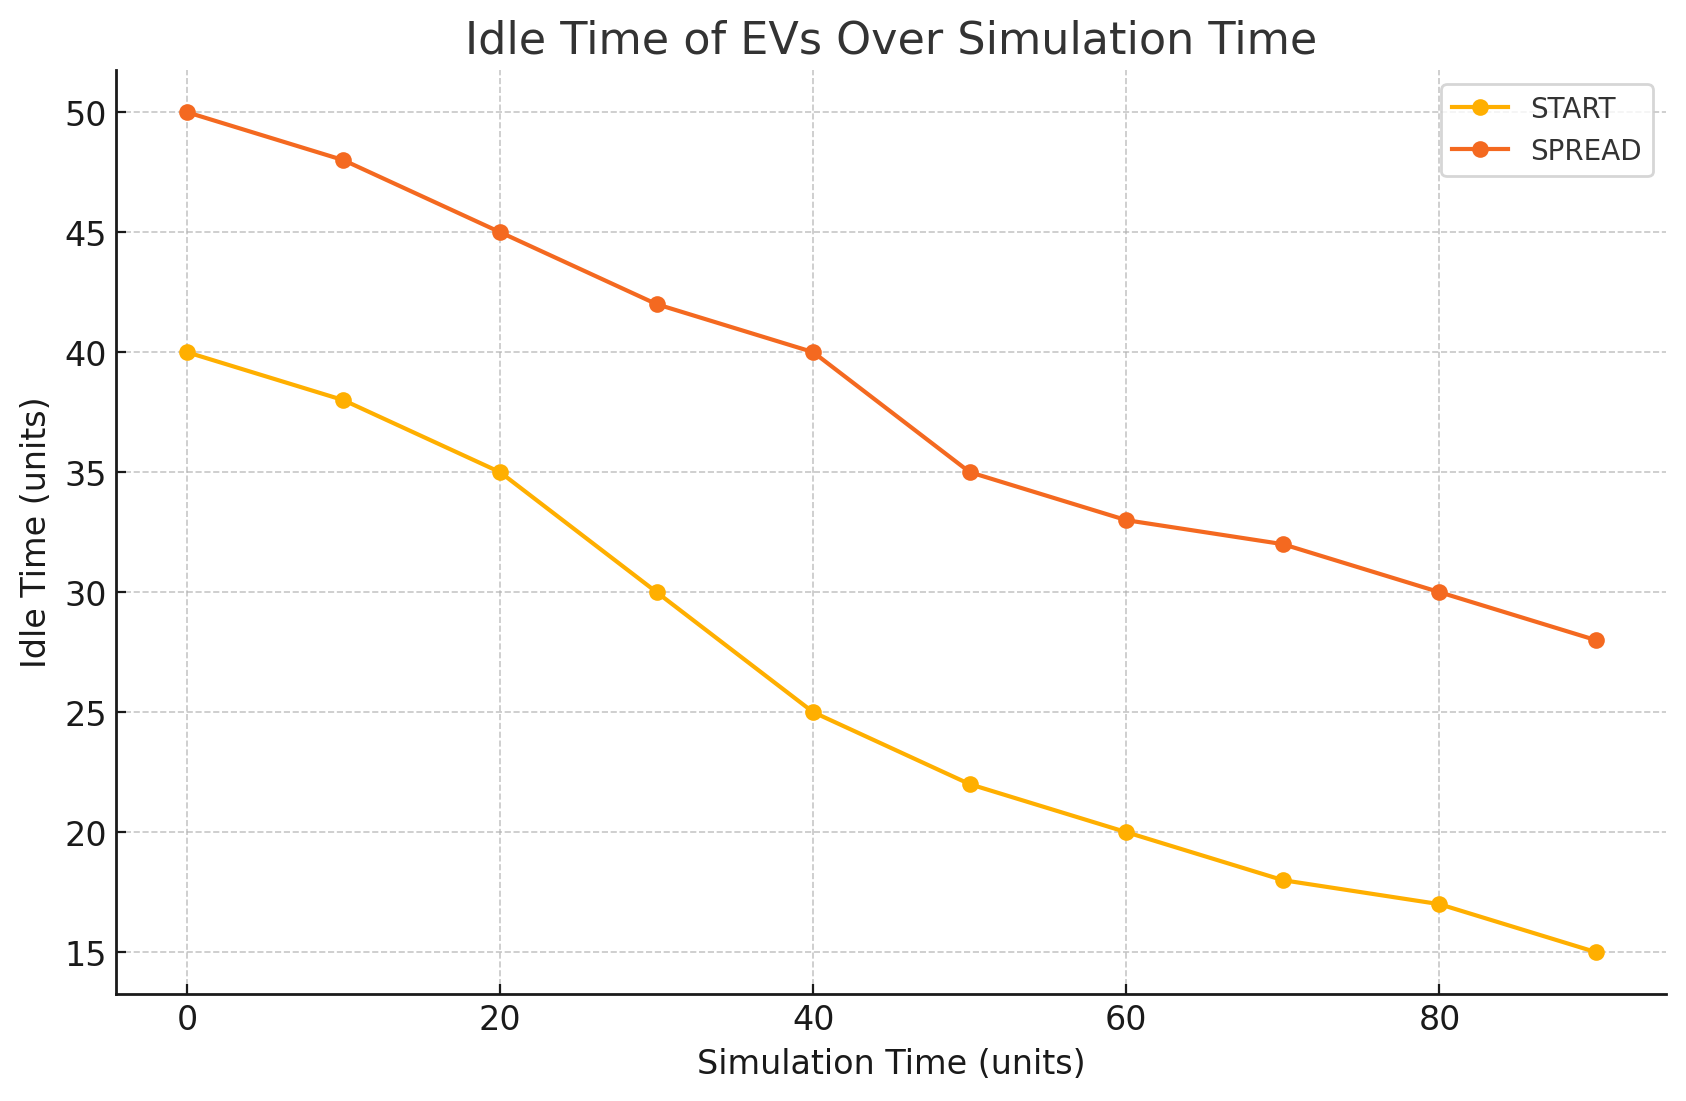
\includegraphics[width=0.8\textwidth]{Crest/Images/idle_time.png}
    \caption{Idle Time of AEVs Over Simulation Time (\%)}
    \label{fig:idle_time_img}
\end{figure}

\begin{table}[h!]
\centering
\begin{tabular}{|c|c|c|}
\hline
\textbf{Simulation Step (\%)} & \textbf{START Mode} & \textbf{SPREAD Mode} \\ \hline
0  & 40  & 50  \\
10 & 38  & 48  \\ 
20 & 35  & 45  \\ 
30 & 30  & 42  \\ 
40 & 25  & 40  \\ 
50 & 22  & 35  \\ 
60 & 20  & 33  \\ 
70 & 18  & 32  \\ 
80 & 17  & 30  \\ 
90 & 15  & 28  \\ \hline
\end{tabular}
\caption{Idle Time of AEVs Over Simulation Time for START vs. SPREAD Modes}
\label{tab:idle_time_tab}
\end{table}


% \subsubsection{Discussion}
The results show that the dispatch mechanism used has a substantial impact on the overall performance of the service. The START option is preferable in scenarios with strong demand early in the simulation. However, the SPREAD mode is more realistic in terms of RES generation, and more applicable in scenarios where resource conservation is crucial.

\subsection{Analysis - SEC Configurations on System Performance}
\label{sec:sec_configurations}

This experiment analyses the performance of the ride-sharing service across several SEC settings. A study of the number and distribution of SECs in various city layouts is done, with an emphasis on TPs served and energy consumption. The ideal configuration is discussed by experimenting with centralised, decentralised, and uneven SEC distributions.

\subsubsection{Experimental Parameters}
Three main SEC configurations are tested:
\begin{itemize}
    \item \textbf{Scenario 1 - Centralised SEC (1 SEC):} One SEC is placed at the centre of the city grid and owns all AEVs. This setup represents a centralised energy system, where all AEVs must return to a single point to recharge.

    \item \textbf{Scenario 2 - Uniformly Decentralised SECs (4 and 16 SECs):} In this scenario, two different configurations are tested. First, four SECs are evenly distributed across the city grid; then, sixteen SECs are also evenly distributed. Both configurations aim to reduce the travel distances of the AEVs and maintain a balanced energy supply across the area. The goal is to understand how increasing the number of uniformly distributed SECs affects system performance.

    \item \textbf{Scenario 3 - Non-uniform SEC Distribution:} This setup has four SECs grouped in one corner of the city grid, as shown in Figure~\ref{fig:non_uniform_sec}. 
\end{itemize}
\begin{figure}[h!]
    \centering
    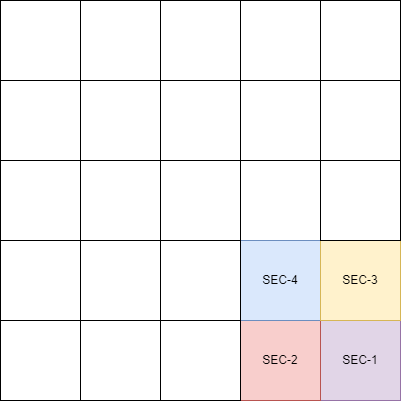
\includegraphics[width=0.5\textwidth, height=0.3\textheight]{Crest/Images/chapter_3_1_non_uniform_sec.png}
    \caption{Non-uniform SEC Distribution}
    \label{fig:non_uniform_sec}
\end{figure}

For each configuration, we test three different energy generation rates at SECs:
\begin{itemize}
    \item \textbf{Low Energy Generation:} Limited energy production, representing energy-scarce environments, 0.5 Energy factor (cf. Section 3.3.1).
    \item \textbf{Medium Energy Generation:} Balanced energy availability across SEC, 1.0 Energy Factor.
    \item \textbf{High Energy Generation:} Abundant energy production, allowing for rapid AEV launch and continuous operation, 2.0 Energy Factor.
\end{itemize}

Tables \ref{tab:trip_satisfaction_sec_refined} and \ref{tab:energy_efficiency_sec_refined} summarise the results of the experiments, comparing different SEC setups and energy generation rates.

Table \ref{tab:trip_satisfaction_sec_refined} and Figures \ref{fig:trip_satisfaction_rate},  \ref{fig:idle_time} show that the completely decentralised SEC configuration (16 SECs, uniformly distributed) has the highest trip satisfaction rate due to the localised position of the SECs, which decreases AEV transit time. The non-uniform distribution of SECs performs the worst, particularly at low energy generation rates, due to unequal vehicle availability.

Table \ref{tab:energy_efficiency_sec_refined} and Figure \ref{fig:energy_utilization} highlight that the centralised architecture (1 SEC) has higher energy efficiency during high energy generation rates (being able to release a good amount of AEVs over time, all of them initially located within reachable distance for any upcoming TP). However, this comes at the cost of having average longer routes for the AEVs. Decentralised arrangements are more suited to TPs due to reduced travel distances.

Table \ref{tab:energy_efficiency_sec_refined} and Figure \ref{fig:average_travel_distance} show that AEVs in the centralised SEC system travel significantly further than those in decentralised arrangements. Non-uniform SEC design result in varying trip distances.

\begin{table}[h!]
\centering
\resizebox{\textwidth}{!}{%
\begin{tabular}{|c|c|c|c|}
\hline
\textbf{SEC Configuration} & \textbf{Trip Satisfaction (\%)} & \textbf{Energy Level} & \textbf{Idle Time} \\ \hline
1 SEC (Centralised)         & 62.3  & Low    & 35 \\
1 SEC (Centralised)         & 70.0  & Medium & 30 \\
1 SEC (Centralised)         & 75.6  & High   & 28 \\
4 SECs (Uniform)            & 68.2  & Low    & 25 \\
4 SECs (Uniform)            & 80.1  & Medium & 22 \\
4 SECs (Uniform)            & 84.5  & High   & 18 \\
16 SECs (Decentralised)     & 78.0  & Low    & 15 \\
16 SECs (Decentralised)     & 85.7  & Medium & 18 \\
16 SECs (Decentralised)     & 89.69 & High   & 12 \\
4 SECs (Non-uniform)        & 50.5  & Low    & 40 \\
4 SECs (Non-uniform)        & 60.0  & Medium & 35 \\
4 SECs (Non-uniform)        & 65.0  & High   & 30 \\ \hline
\end{tabular}%
}
\caption{Trip Satisfaction Rate and Idle Time Across SEC Configurations and Energy Generation Levels}
\label{tab:trip_satisfaction_sec_refined}
\end{table}


\begin{table}[h!]
\centering
\resizebox{\textwidth}{!}{%
\begin{tabular}{|c|c|c|c|}
\hline
\textbf{SEC Configuration} & \textbf{Energy Utilised} & \textbf{Energy Level} & \textbf{Average Travel Distance} \\ \hline
1 SEC (Centralised)         & 8.5   & Low    & 95 \\
1 SEC (Centralised)         & 8.0   & Medium & 85 \\
1 SEC (Centralised)         & 7.9   & High   & 80 \\
4 SECs (Uniform)            & 7.8   & Low    & 70 \\
4 SECs (Uniform)            & 7.2   & Medium & 60 \\
4 SECs (Uniform)            & 6.9   & High   & 55 \\
16 SECs (Decentralised)     & 6.8   & Low    & 50 \\
16 SECs (Decentralised)     & 7.0   & Medium & 45 \\
16 SECs (Decentralised)     & 6.5   & High   & 40 \\
4 SECs (Non-uniform)        & 9.1   & Low    & 110 \\
4 SECs (Non-uniform)        & 8.5   & Medium & 95 \\
4 SECs (Non-uniform)        & 8.0   & High   & 90 \\ \hline
\end{tabular}%
}
\caption{Energy Utilisation and Average Travel Distance Across SEC Configurations and Energy Levels}
\label{tab:energy_efficiency_sec_refined}
\end{table}


% \begin{table}[h!]
% \centering
% \begin{tabular}{|c|c|c|}
% \hline
% \textbf{SEC} & \textbf{Average Travel Distance } & \textbf{Energy } \\ \hline
% 1 SEC (Centralised)         & 95   & Low    \\ 
% 1 SEC (Centralised)         & 80   & High   \\ 
% 4 SECs (Uniform)            & 60   & Medium \\ 
% 4 SECs (Non-uniform)        & 110  & Low    \\ 
% 16 SECs (Decentralised)     & 40   & High   \\ 
% 16 SECs (Decentralised)     & 45   & Medium \\ \hline
% \end{tabular}
% \caption{Average Travel Distance Across SEC Configurations and Energy Generation Rates}
% \label{tab:travel_distance_sec_refined}
% \end{table}

\begin{figure}[h!]
    \centering
    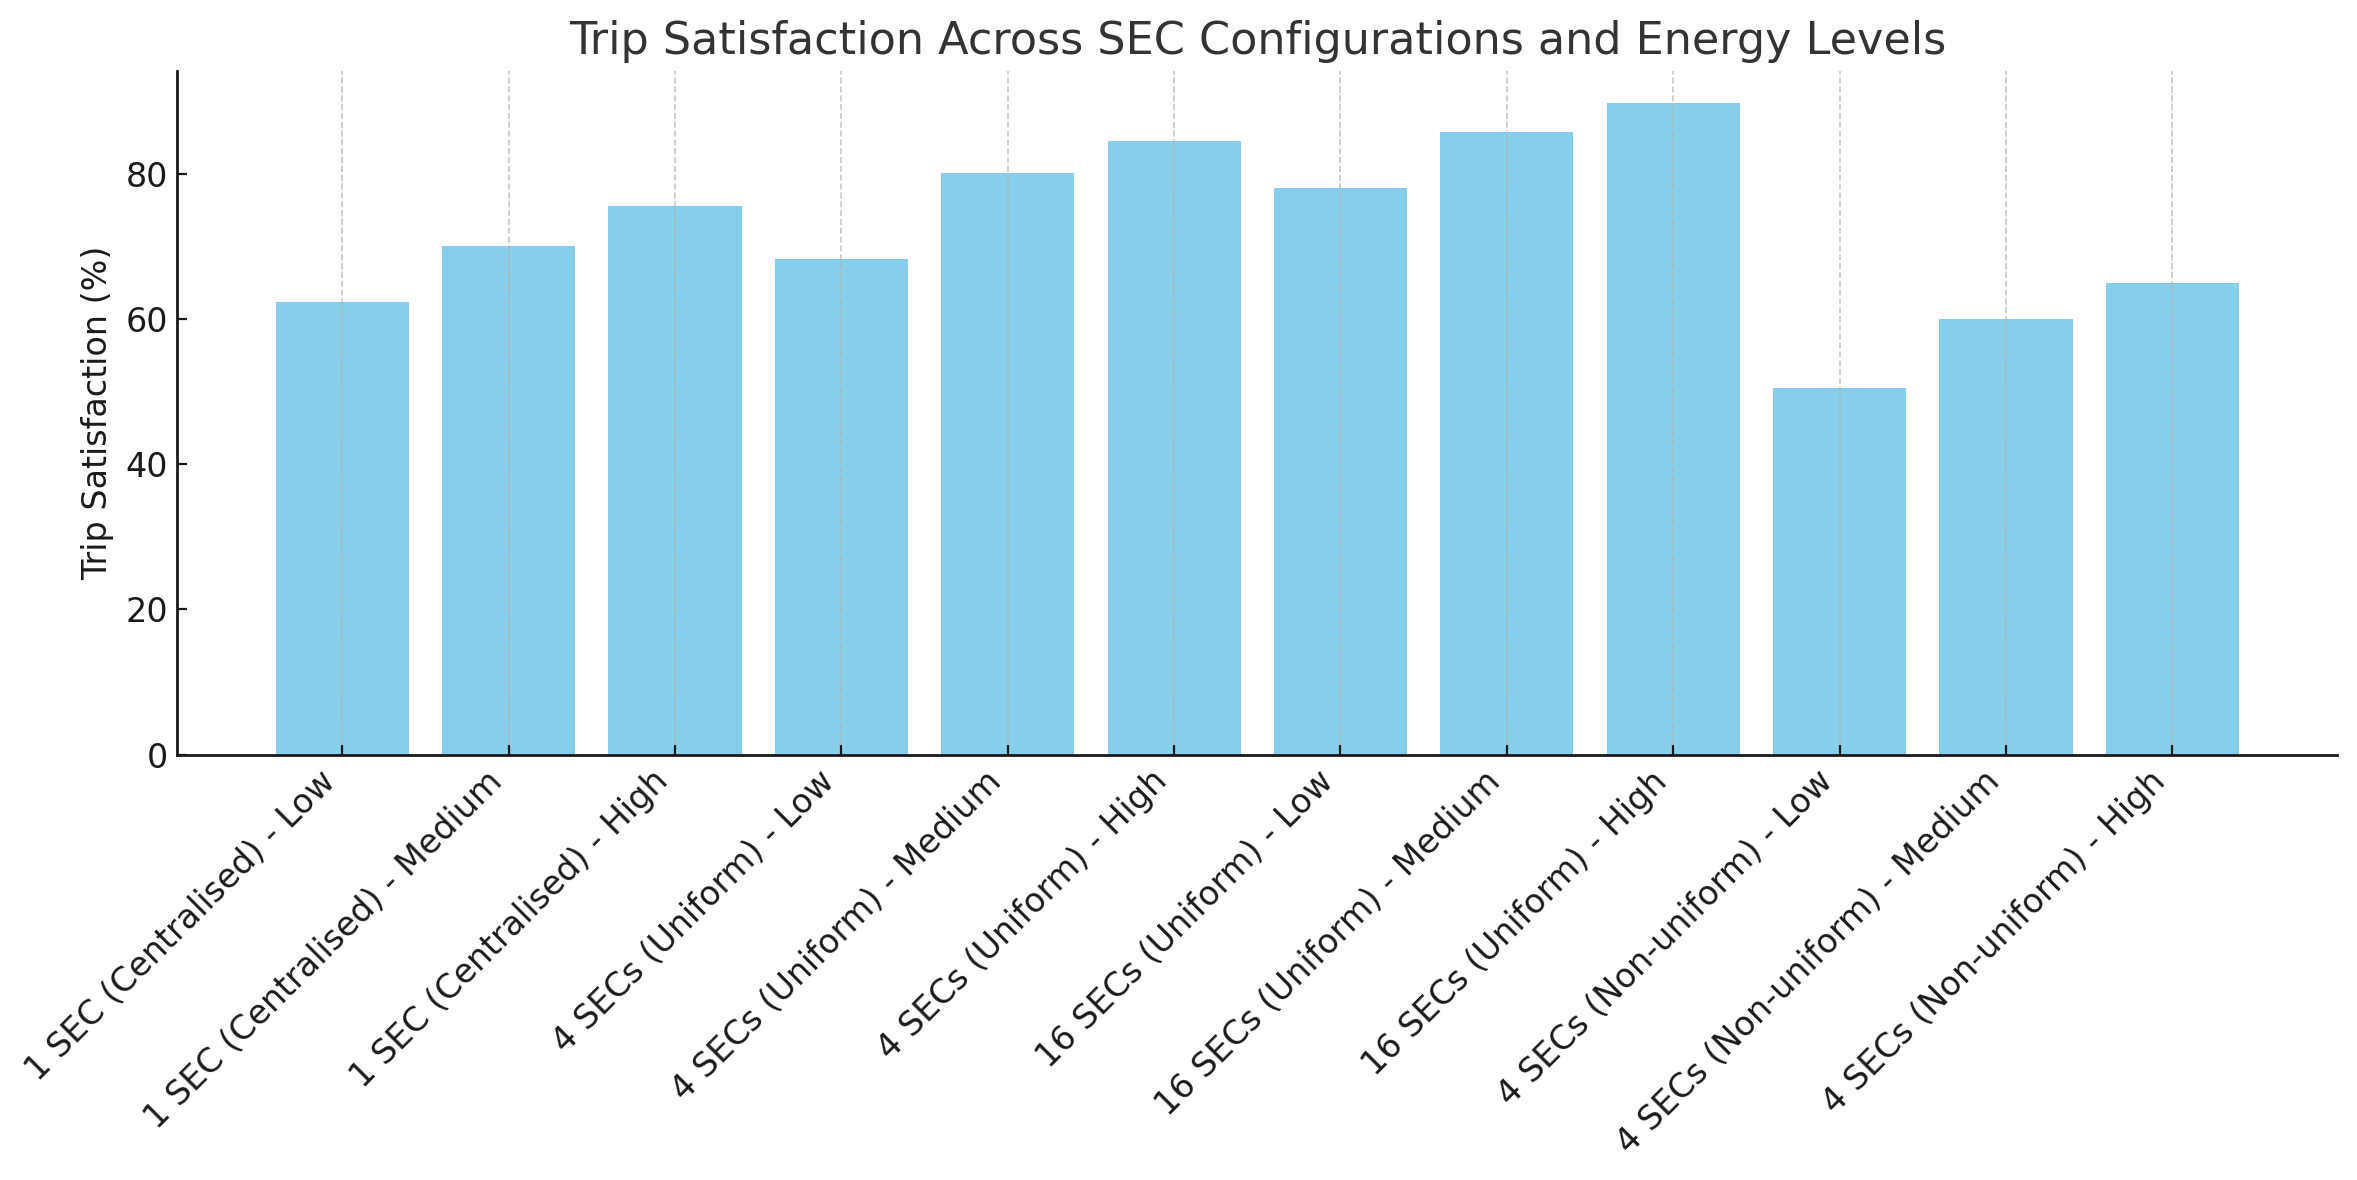
\includegraphics[width=0.8\textwidth]{Crest/Images/trip_satisfaction_rate.png}
    \caption{Trip Satisfaction Rate Over Simulation Time for Different SEC Configurations}
    \label{fig:trip_satisfaction_rate}
\end{figure}

\begin{figure}[h!]
    \centering
    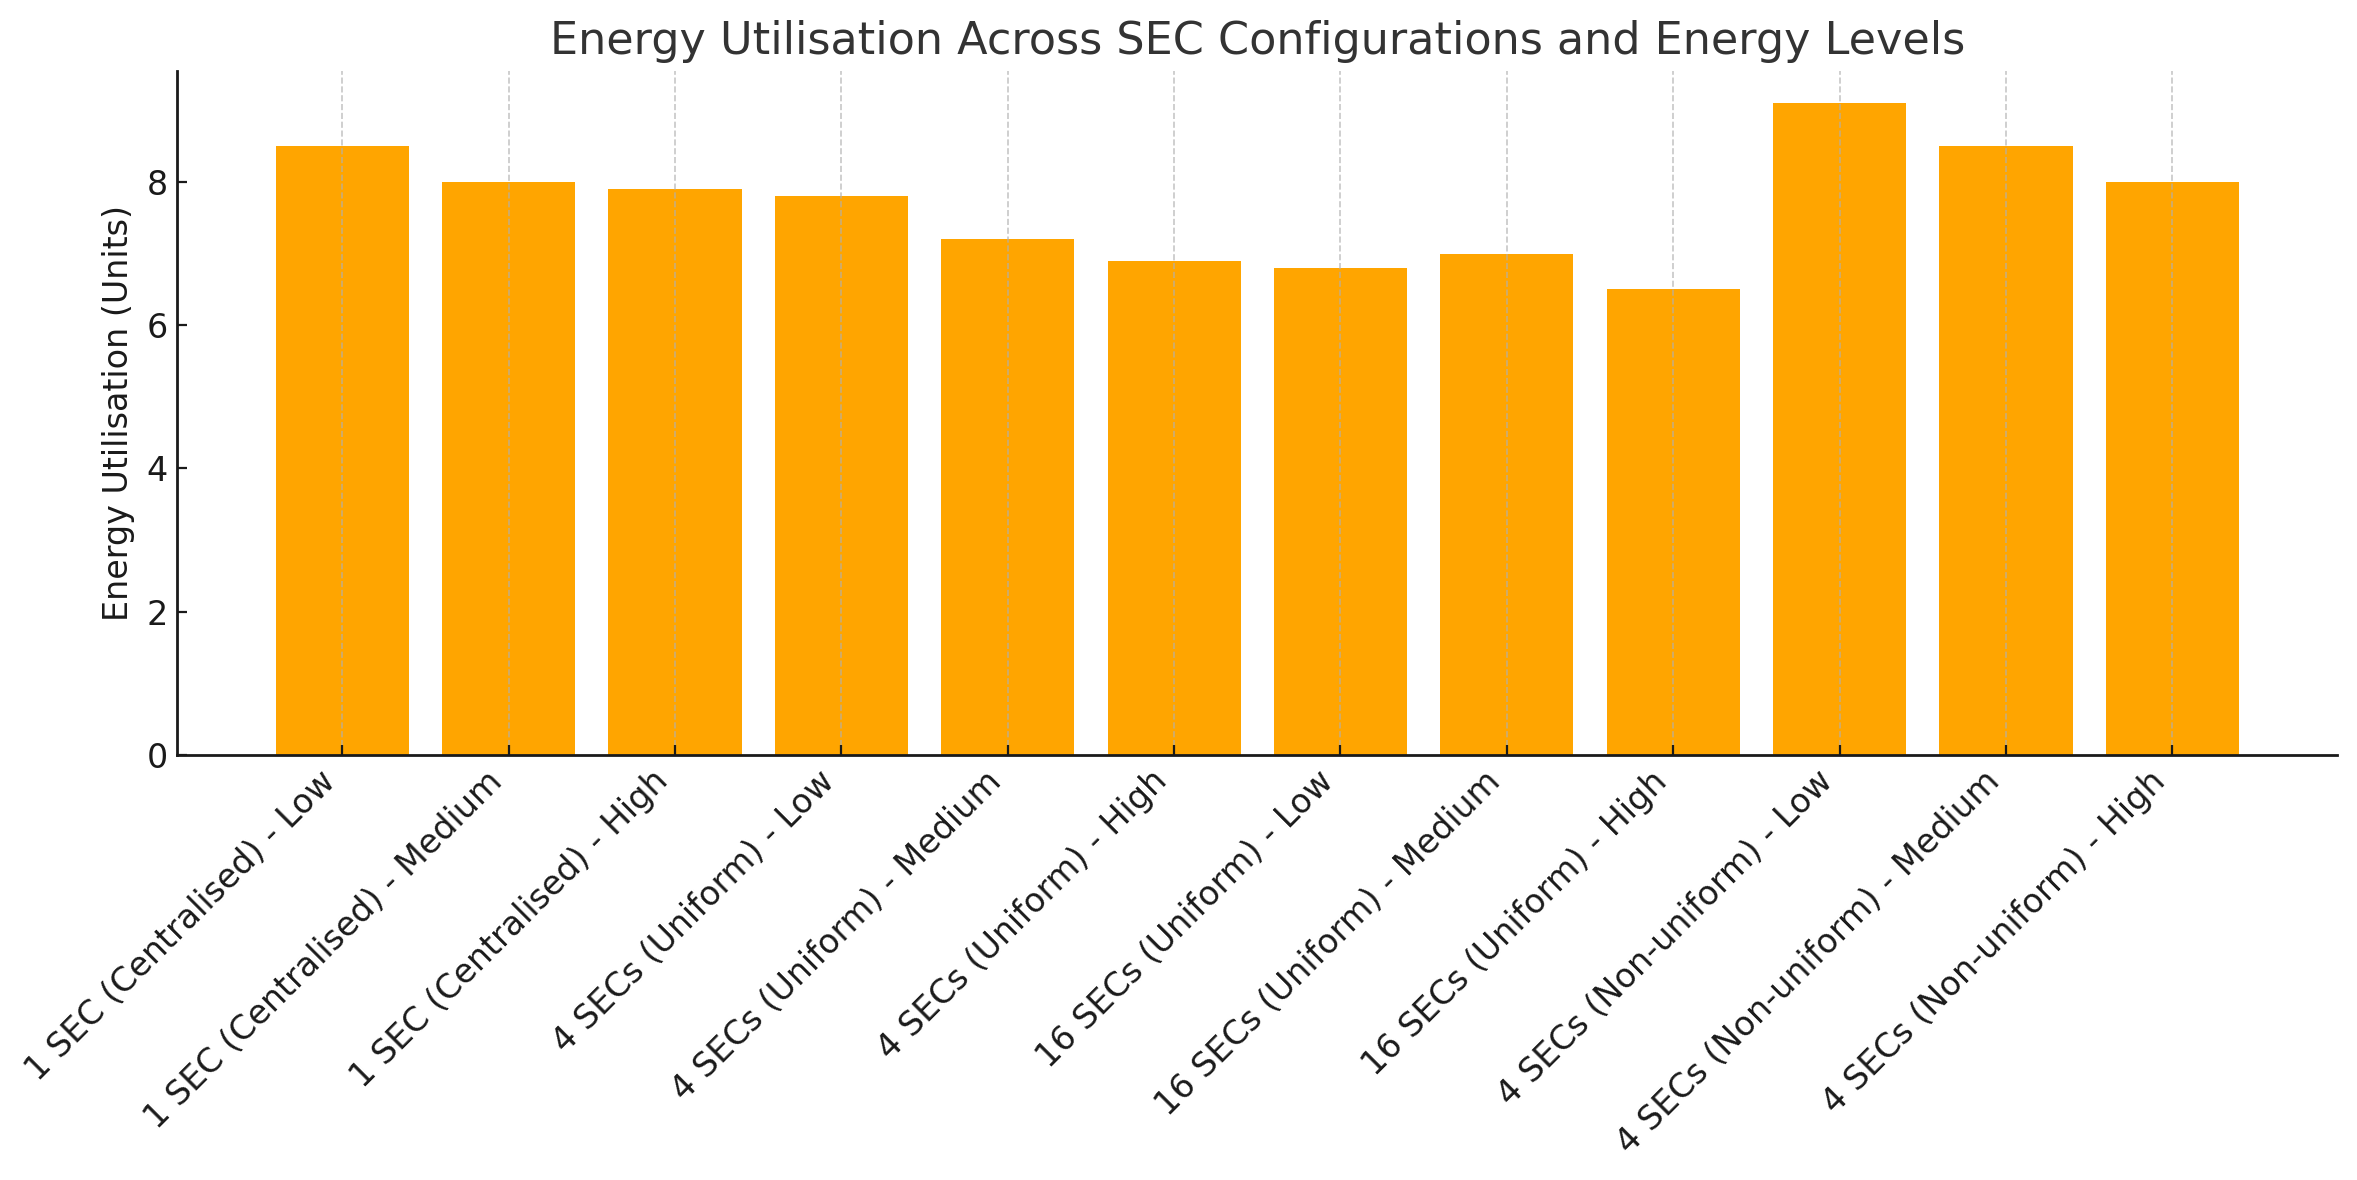
\includegraphics[width=0.8\textwidth]{Crest/Images/energy_utilisation.png}
    \caption{Energy Utilization Over Simulation Time for Different SEC Configurations}
    \label{fig:energy_utilization}
\end{figure}

\begin{figure}[h!]
    \centering
    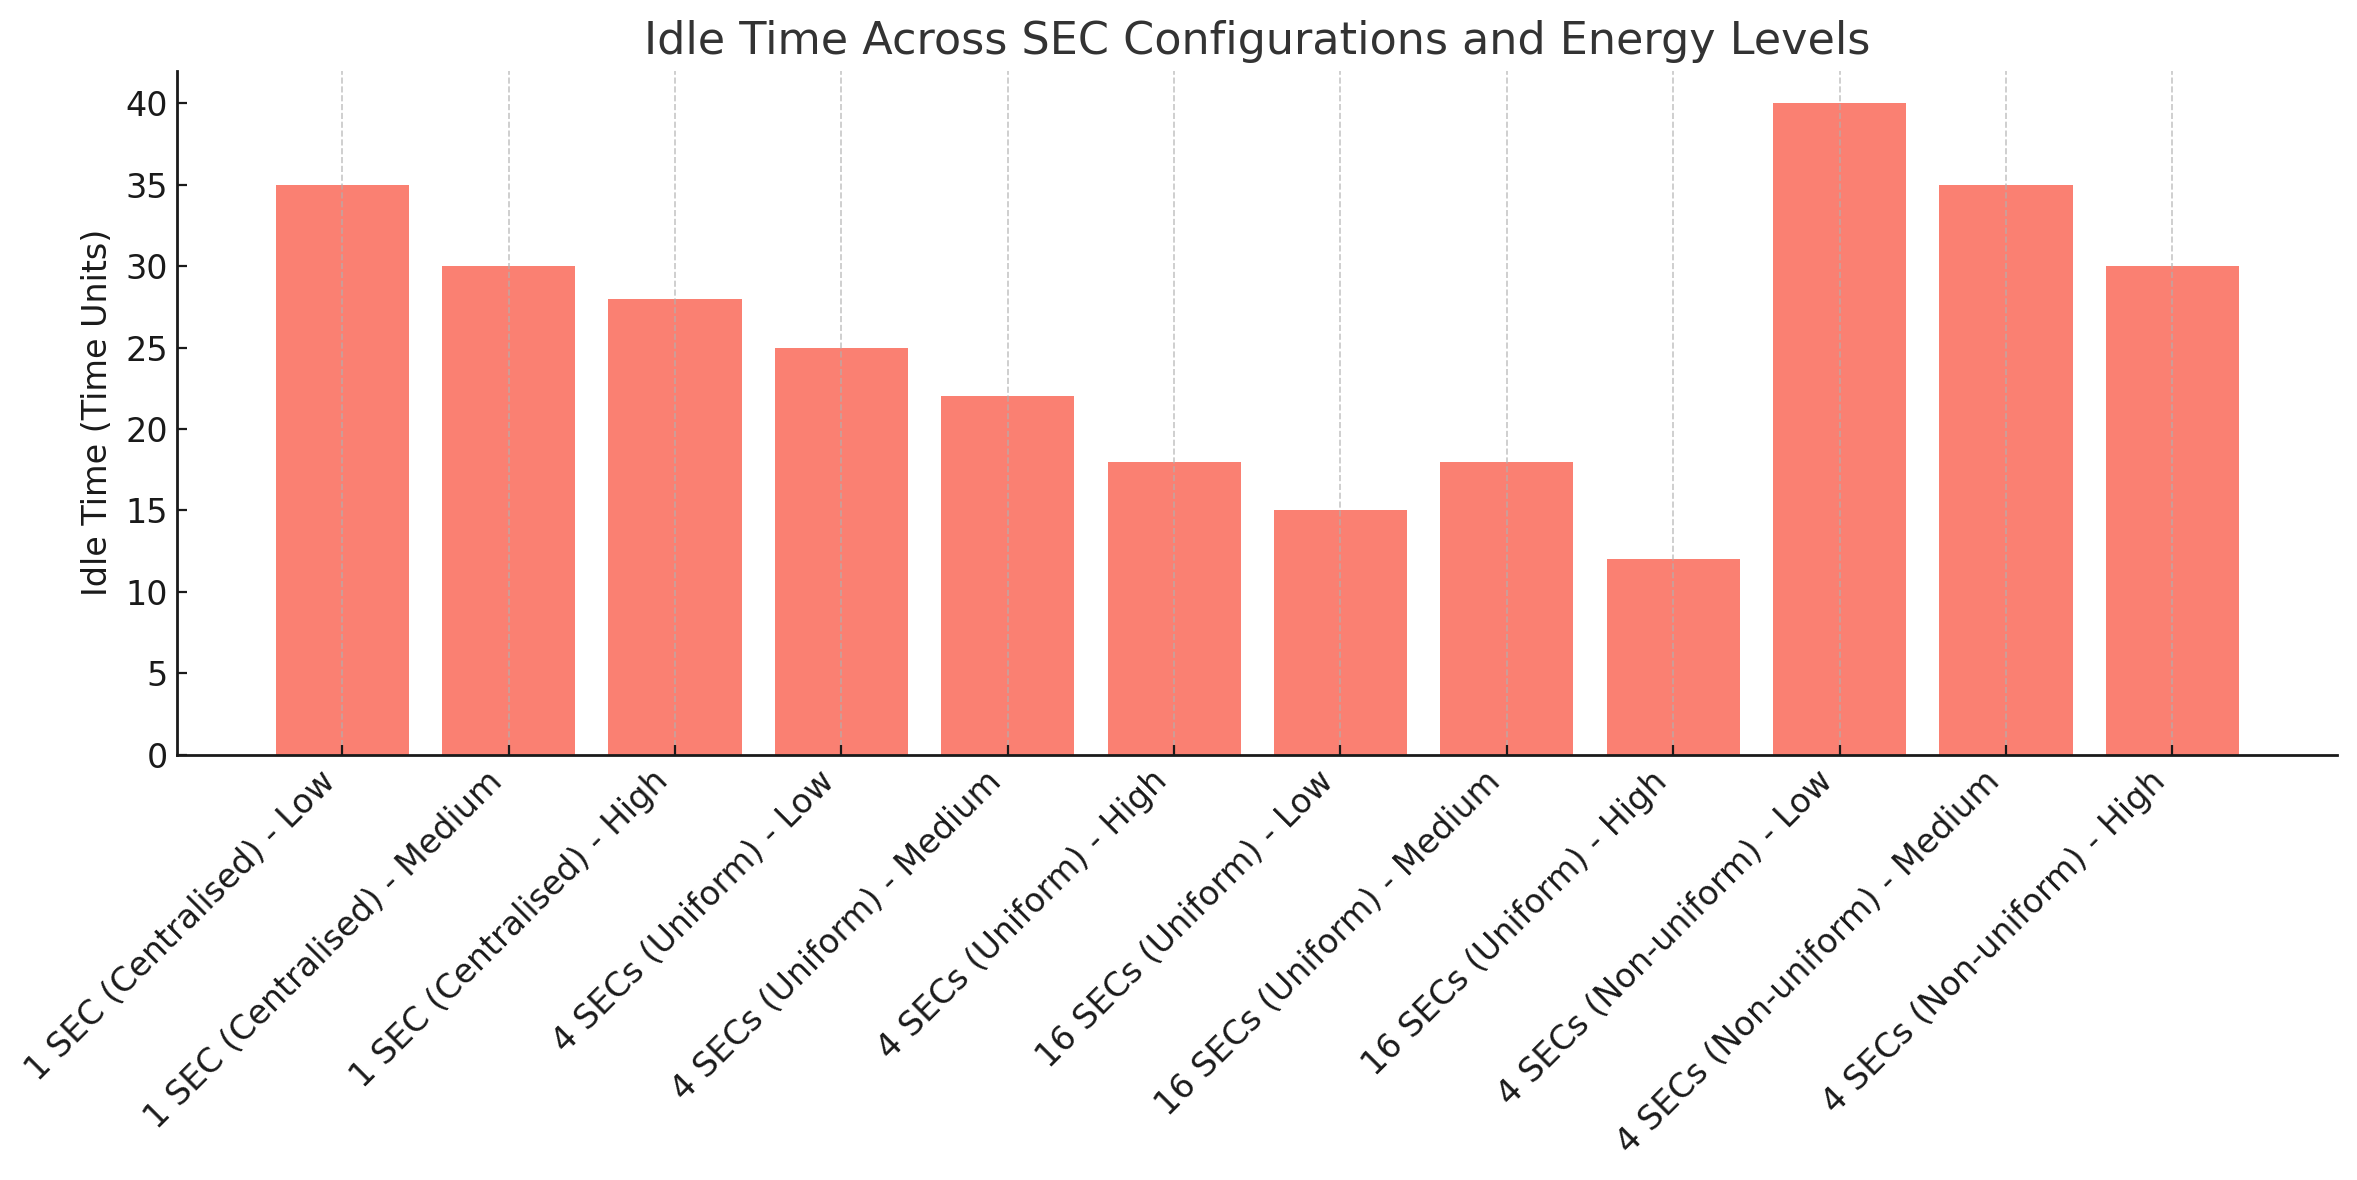
\includegraphics[width=0.8\textwidth]{Crest/Images/idle_time_sec_config.png}
    \caption{Idle Time Over Simulation Time for Different SEC Configurations}
    \label{fig:idle_time}
\end{figure}

\begin{figure}[h!]
    \centering
    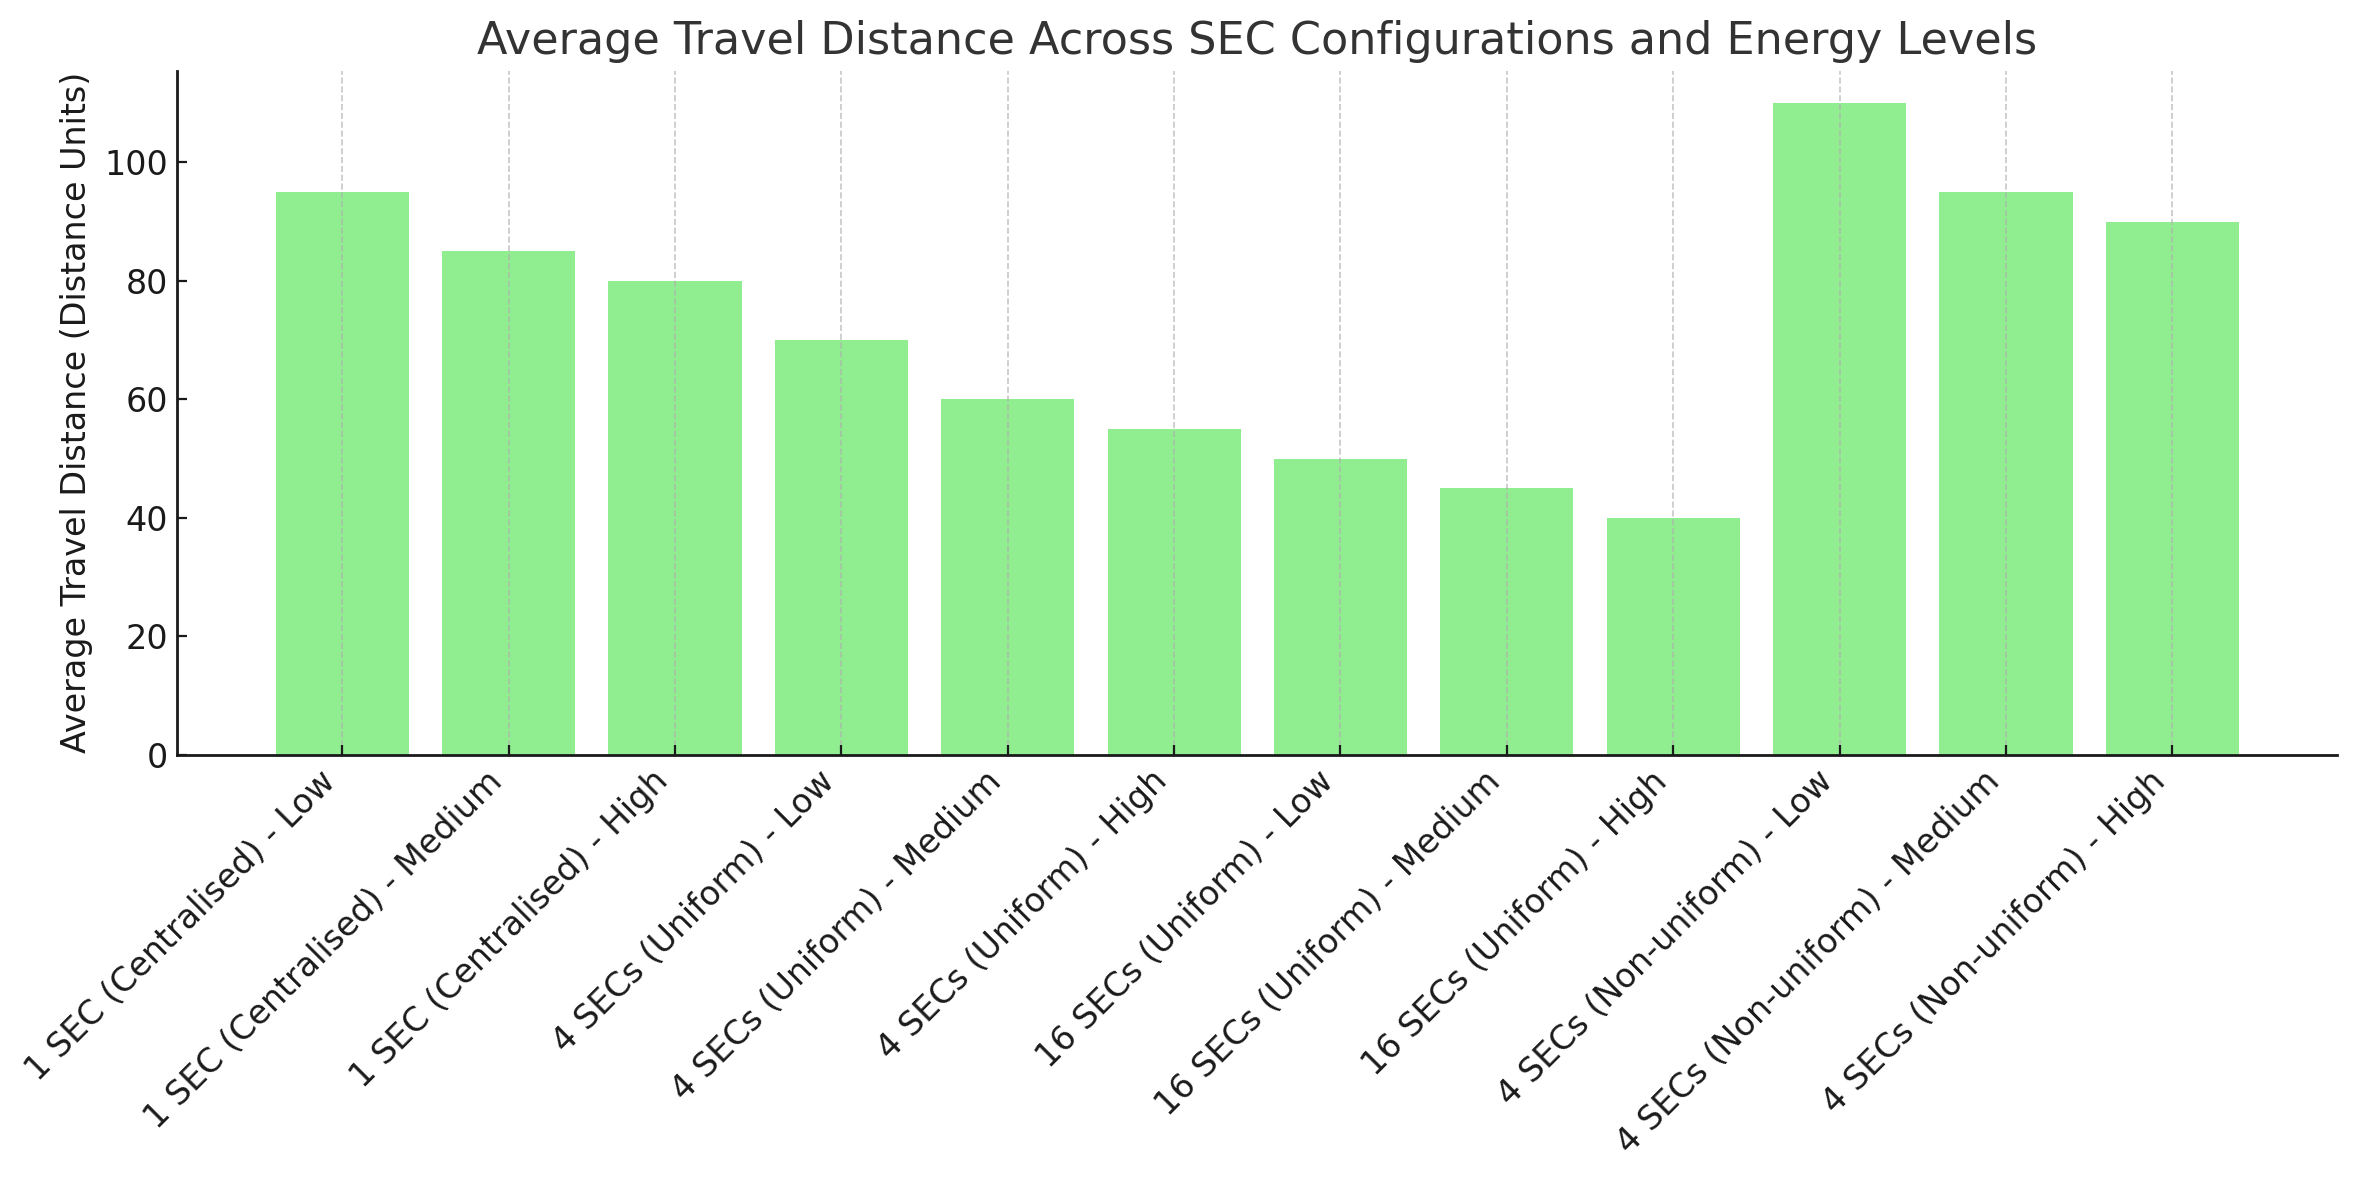
\includegraphics[width=0.8\textwidth]{Crest/Images/average_travel_distance.png}
    \caption{Average Travel Distance Over Simulation Time for Different SEC Configurations}
    \label{fig:average_travel_distance}
\end{figure}

The results show that decentralised SEC configurations, particularly those with uniform distribution, provide the highest overall performance in terms of TP served, energy consumption, and travel distances. In contrast, centralised SEC configurations, have longer travel times, making them less suitable for large city grids. Non-uniform SEC distributions produce the poorest performance due to uneven energy availability and inefficient vehicle placement.

The trade-off between centralised and decentralised systems is mostly determined by city size and energy generation capacity. For smaller cities with limited geographic spread, a centralised SEC arrangement may be adequate. However, in larger cities, decentralised designs, particularly those with uniform distribution, yield substantially superior results.


\section{Conclusions}
\label{sec:conclusion}
This chapter has presented the design, implementation, and evaluation of a carbon-neutral, community-based, reactive ride-sharing service for a smart city with 100\% AEVs operating solely over RES.  

The ride-sharing service has been formulated as a variant of the classical Dynamic Vehicle Routing Problem with Time Windows, with both dynamic resources and requests. The objective function has been set to maximise the overall number of TPs being served. The problem has been solved via a reactive-based simulation approach on top of a greedy-based decision-making process.  

An instance generator has been developed to create configurable scenarios to evaluate the proposed approach. It was used to extend existing benchmarks (Google HashCode) and public datasets (NYC taxis) to the problem formulation and testing the proposed algorithm under different settings. 

The ride-sharing service has proven to scale well,  with a quadratic algorithm complexity over its number of trips, allowing to solve an instance of about 1,000 trips in less than a second, and an instance of about 10,000 trips in less than two minutes.  Although favouring scalability over optimality, the service has proven to be able to solve up to ~90\% of the instances for some configurations of $d\_metropolis.in$, a complex instance from the Google HashCode.  
When applied to the real-world data-set of the NYC taxis and compared to an individual private transportation, the ride-sharing approach has been proven to offer a good trade-off between the amount of vehicles reduced (84\%) and its overhead in terms of distance traversed (21\%). The complete code can be accessed via GitHub \cite{smartgreenscode}. 